\documentclass[acmsmall,review,nonacm]{acmart}

\usepackage{cleveref}
\usepackage{macros}
\usepackage{hott}
\usepackage{quiver}

%% Some recommended packages.
%% \usepackage{booktabs}   %% For formal tables:
                        %% http://ctan.org/pkg/booktabs
%% \usepackage{subcaption} %% For complex figures with subfigures/subcaptions
                        %% http://ctan.org/pkg/subcaption
%% \usepackage{verbatim}
%% \usepackage{amsmath,amsbsy}
%% \usepackage{alltt}
%% \usepackage{fdsymbol}
%% \usepackage{amsthm,proof}
%% \usepackage{bbold,stmaryrd,bbm}
\usepackage{bbold}
%% \usepackage{ucs}
%% \usepackage{wrapfig}
%% \usepackage[utf8x]{inputenc}
%% \usepackage{newunicodechar}
%% \usepackage{microtype}
%% \usepackage{subcaption}
%% \usepackage{agda}
\usepackage{tikz}
\usetikzlibrary{cd}
\usetikzlibrary{quotes}
\usetikzlibrary{decorations.markings}
\usetikzlibrary{knots}
% \usepackage{tikzit}
% ../paper/tikzit.sty

\newtheorem{theorem}{Theorem}
\newtheorem{corollary}[theorem]{Corollary}
\newtheorem{lemma}[theorem]{Lemma}
\newtheorem{definition}[theorem]{Definition}
\newtheorem*{remark}{Remark}

\newcommand{\zerot}{\mathbb{0}}
\newcommand{\onet}{\mathbb{1}}
\newcommand{\sumt}{\mathbin{\mathsf{+}}}
\newcommand{\prodt}{\mathbin{\mathsf{\times}}}
\newcommand{\isot}{\leftrightarrow}

%%
%% \BibTeX command to typeset BibTeX logo in the docs
\AtBeginDocument{%
  \providecommand\BibTeX{{%
    \normalfont B\kern-0.5em{\scshape i\kern-0.25em b}\kern-0.8em\TeX}}}

%% Rights management information.  This information is sent to you
%% when you complete the rights form.  These commands have SAMPLE
%% values in them; it is your responsibility as an author to replace
%% the commands and values with those provided to you when you
%% complete the rights form.
\setcopyright{acmcopyright}
\copyrightyear{2018}
\acmYear{2018}
\acmDOI{10.1145/1122445.1122456}

%% These commands are for a PROCEEDINGS abstract or paper.
\acmConference[Woodstock '18]{Woodstock '18: ACM Symposium on Neural
  Gaze Detection}{June 03--05, 2018}{Woodstock, NY}
\acmBooktitle{Woodstock '18: ACM Symposium on Neural Gaze Detection,
  June 03--05, 2018, Woodstock, NY}
\acmPrice{15.00}
\acmISBN{978-1-4503-XXXX-X/18/06}


%%
%% Submission ID.
%% Use this when submitting an article to a sponsored event. You'll
%% receive a unique submission ID from the organizers
%% of the event, and this ID should be used as the parameter to this command.
%%\acmSubmissionID{123-A56-BU3}

%%
%% The majority of ACM publications use numbered citations and
%% references.  The command \citestyle{authoryear} switches to the
%% "author year" style.
%%
%% If you are preparing content for an event
%% sponsored by ACM SIGGRAPH, you must use the "author year" style of
%% citations and references.
%% Uncommenting
%% the next command will enable that style.
\citestyle{acmauthoryear}

%%
%% end of the preamble, start of the body of the document source.
\begin{document}

%%
%% The "title" command has an optional parameter,
%% allowing the author to define a "short title" to be used in page headers.
\title{Reversible Programming with Univalent Finite Types}

%%
%% The "author" command and its associated commands are used to define
%% the authors and their affiliations.
%% Of note is the shared affiliation of the first two authors, and the
%% "authornote" and "authornotemark" commands
%% used to denote shared contribution to the research.
\author{Anonymous}

%%
%% By default, the full list of authors will be used in the page
%% headers. Often, this list is too long, and will overlap
%% other information printed in the page headers. This command allows
%% the author to define a more concise list
%% of authors' names for this purpose.
\renewcommand{\shortauthors}{Anonymous}

%%
%% The abstract is a short summary of the work to be presented in the
%% article.
\begin{abstract}
  We establish a close connection between a reversible programming language
  based on isomorphisms of finite types and a formally presented univalent
  universe.

  The correspondence relates combinators witnessing type isomorphisms in the
  programming language to paths in the univalent universe; and combinator
  optimisations in the programming language to 2-paths in the univalent
  universe.

  The main result is a \ldots
\end{abstract}

%%
%% The code below is generated by the tool at http://dl.acm.org/ccs.cfm.
%% Please copy and paste the code instead of the example below.
%%
\begin{CCSXML}
  <ccs2012>
   <concept>
       <concept_id>10003752.10003790.10011740</concept_id>
       <concept_desc>Theory of computation~Type theory</concept_desc>
       <concept_significance>500</concept_significance>
       </concept>
   <concept>
       <concept_id>10003752.10010124.10010131.10010137</concept_id>
       <concept_desc>Theory of computation~Categorical semantics</concept_desc>
       <concept_significance>500</concept_significance>
       </concept>
   <concept>
       <concept_id>10003752.10010124.10010131.10010133</concept_id>
       <concept_desc>Theory of computation~Denotational semantics</concept_desc>
       <concept_significance>500</concept_significance>
       </concept>
   <concept>
       <concept_id>10011007.10011006.10011008.10011009.10011012</concept_id>
       <concept_desc>Software and its engineering~Functional languages</concept_desc>
       <concept_significance>500</concept_significance>
       </concept>
   <concept>
       <concept_id>10011007.10011006.10011039.10011040</concept_id>
       <concept_desc>Software and its engineering~Syntax</concept_desc>
       <concept_significance>500</concept_significance>
       </concept>
   <concept>
       <concept_id>10011007.10011006.10011039.10011311</concept_id>
       <concept_desc>Software and its engineering~Semantics</concept_desc>
       <concept_significance>500</concept_significance>
       </concept>
 </ccs2012>
\end{CCSXML}

\ccsdesc[500]{Theory of computation~Type theory}
\ccsdesc[500]{Theory of computation~Categorical semantics}
\ccsdesc[500]{Theory of computation~Denotational semantics}
\ccsdesc[500]{Software and its engineering~Functional languages}
\ccsdesc[500]{Software and its engineering~Syntax}
\ccsdesc[500]{Software and its engineering~Semantics}

%%
%% Keywords. The author(s) should pick words that accurately describe
%% the work being presented. Separate the keywords with commas.
\keywords{reversible computing}

%%
%% This command processes the author and affiliation and title
%% information and builds the first part of the formatted document.
\maketitle

%%%%%%%%%%%%%%%%%%%%%%%%%%%%%%%%%%%%%%%%%%%%%%%%%%%%%%

\section{Introduction}~\label{sec:introduction}

\paragraph*{Synthesis of Reversible Core of Quantum Circuits.} Most current quantum algorithms start with generating superpositions, evolving them using a unitary transformation, and then projecting them with a measurement operator. The middle stage is essentially a reversible classical computation (executed in a quantum-parallel fashion). We illustrate that middle stage in detail by synthesizing a reversible circuit implementing boolean disjunction ($\vee$). Following~\citet{Toffoli:1980}, the first step is to write a specification for the desired reversible function:
\[
\mathit{reversibleOr}(h,b_1,b_2) ~=~ (h \,\underline{\vee}\, (b_1 \vee b_2), ~b_1, ~b_2)
\]
where $\underline{\vee}$ is the exclusive-or operation. From the definition of $\underline{\vee}$ it is evident that setting $h=0$, we can compute the desired disjunction by observing the first component of the result. The $\mathit{reversibleOr}$ function has the following truth table (in binary on the left and in a more convenient decimal notation on the right):

\begin{center}\begin{tabular}{|ccc|ccc|@{\qquad\qquad}|c|c|}
0 & 0 & 0 &     0 & 0 & 0     & 0 & 0 \\
0 & 0 & 1 &     1 & 0 & 1     & 1 & 5 \\
0 & 1 & 0 &     1 & 1 & 0    & 2 & 6 \\
0 & 1 & 1 &     1 & 1 & 1    & 3 & 7 \\
1 & 0 & 0 &     1 & 0 & 0    & 4 & 4 \\
1 & 0 & 1 &     0 & 0 & 1    & 5 & 1 \\
1 & 1 & 0 &     0 & 1 & 0    & 6 & 2 \\
1 & 1 & 1 &     0 & 1 & 1    & 7 & 3
\end{tabular}\end{center}

\noindent where it is evident that it is a bijective function, i.e., reversible.

The above embedding of an irreversible function into a reversible function with additional inputs and outputs is completely general and is the starting point for specifications of quantum circuits. The challenge is to synthesize a program / circuit from this specification. Of course, writing this program in a conventional (irreversible) language defeats the purpose. The challenge is to construct the desired program / circuit exclusively using reversible primitives, e.g., the standard set of universal reversible gates used in frameworks like Qiskit which consists of the computational gates \textsf{not} (boolean negation, called \verb|x|), \textsf{cnot} (conditional negation of the second input if the first is true; called \verb|cx|), and \textsf{toffoli} (conditional negation of the third input if both the first two inputs are true; called \verb|ccx|) gates, and the ability re-arrange the layout of wires. For concreteness, here is a possible implementation of the desired function in Qiskit:

\begin{center}
  \begin{minipage}[c]{0.4\linewidth}
\begin{verbatim}
reversibleOr.qasm:

  // setup
  ccx q[1], q[2], q[0];
  cx  q[1], q[0];
  cx  q[2], q[0];
  // measure

% ./qasm -t reversibleOr.qasm
+-------+-------+
| 0 0 0 | 0 0 0 |
| 0 0 1 | 1 0 1 |
| 0 1 0 | 1 1 0 |
| 0 1 1 | 1 1 1 |
| 1 0 0 | 1 0 0 |
| 1 0 1 | 0 0 1 |
| 1 1 0 | 0 1 0 |
| 1 1 1 | 0 1 1 |
+-------+-------+
  \end{verbatim}
  \end{minipage}
  \qquad
  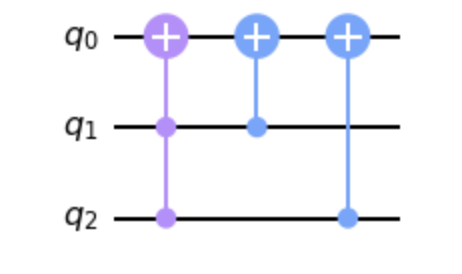
\includegraphics[scale=0.7]{reversibleOr.png}
\end{center}

\noindent This implementation was manually produced using a standard synthesis algorithm for reversible
circuits~\cite{10.1145/775832.775915}. To gain some intuition, we trace the evaluation of the circuit for input
\verb|011|. In this context, the most significant bit is at index 0. Thus the first \verb|ccx| gate negates \verb|q[0]|
since both \verb|q[1]| and \verb|q[2]| are true producing \verb|111|; the following \verb|cx| gate produces \verb|011|; finally the last \verb|cx| produces the result \verb|111|.

There is wealth of manual and algorithmic approaches for such synthesis problems each optimizing along  different dimensions~\cite{XXX}. Here is the circuit produced using an approach that analyzes the recursive structure of the circuit (and would generalize to computing the disjunction of more than two inputs):

\begin{center}
  \begin{minipage}[c]{0.4\linewidth}
\begin{verbatim}
reversibleOr2.qasm:

  // setup
  cx  q[1], q[0];
  x   q[1];
  ccx q[1], q[2], q[0];
  x   q[1];
  // measure
  \end{verbatim}
  \end{minipage}
  \qquad
  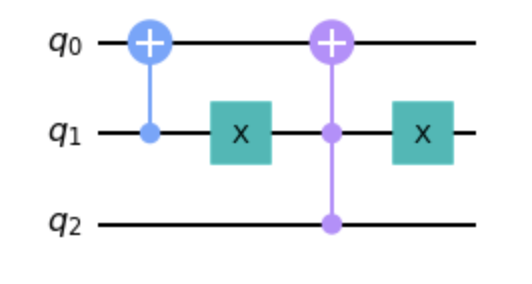
\includegraphics[scale=0.7]{reversibleOr2.png}
\end{center}

\noindent The evaluation of this circuit prints the same truth table as above confirming their equivalence. Tracing the
evaluation on the same input value \verb|011| goes through the stages \verb|111|, \verb|101|, \verb|101|, and finally \verb|111|.

The situation for Shor's algorithm is just as described above but with a more involved function of the form $f(r) = a^{r} \mod N$ for fixed $a$ and $N$. The specification of the circuit is relatively straightforward to calculate. Here it is for $a=11$ and $N=15$:
\[\begin{array}{rcll}
g(r,h) &=& \left\{ \begin{array}{ll}
                     (r,h+1) & \mbox{when~$r$~even~and~$h$~even} \\
                     (r,h-1) & \mbox{when~$r$~even~and~$h$~odd} \\
                     (r,11-h) & \mbox{when~$r$~odd~and~$4 > h \geq 0$~or~$12 > h \geq 8$} \\
                     (r,19-h) & \mbox{when~$r$~odd~and~$8 > h \geq 4$~or~$16 > h \geq 12$}
                                \end{array}\right.
\end{array}\]

\noindent However, as explained in standard accounts of the algorithm (e.g., the Qiskit implementation), producing an efficient
modular exponentiation circuit from this specification  is not straightforward and is actually the bottleneck in Shor’s algorithm. Typical
derivations of the circuit start from elementary gates, build a circuit for reversible disjunction and conjunction of
booleans, a circuit for a half-adder, a circuit for computing the carry, progressing to a circuit for modular addition,
which is used to build a circuit for modular multiplication, and then finally a circuit for modular exponentiation
taking care at each step to avoid the exponential blowup (e.g., by implementing exponentiation by squaring instead of repeated
multiplication)~\cite{shorefficient}.

\paragraph*{Our Technical Results.} The main result of the paper is a proof, formalized in the HoTT-Agda library, that
the category of finite sets and bijections is the free rig groupoid; its structure is illustrated diagrammatically below:

\[\begin{tikzcd}
    \PiLang && \PiPlusLang && \PiHatLang && \UFin
    \arrow["\evalt", from=1-1, to=1-3]
    \arrow["\evalp", curve={height=-24pt}, from=1-3, to=1-5]
    \arrow["\evalh", curve={height=-24pt}, from=1-5, to=1-7]
    \arrow["\quotep", curve={height=-24pt}, from=1-5, to=1-3]
    \arrow["\quoteh", curve={height=-24pt}, from=1-7, to=1-5]
  \end{tikzcd}\]

\noindent The nodes $\PiLang$, $\PiPlusLang$, and $\PiHatLang$ in the diagram each represent a syntactic weak 2-category
(groupoid actually as all morphisms are isomorphisms) where the 0-cells represent types, the 1-cells represent
reversible circuits, and the 2-cells represent circuit equivalences. In $\PiLang$, the circuits represent arbitrary
permutations among finite sets with products and coproducts; in $\PiPlusLang$, the circuits represent arbitrary
permutations among finite sets with only coproducts; and in $\PiHatLang$, the permutations are expressed using adjacent
transpositions.

The syntactic groupoid $\PiPlusLang$ is the free rig groupoid; $\UFin$ is the groupoid of finite sets and bijections
represented as the \emph{univalent subuniverse of all finite types}. The $\evalp/\quotep$ and $\evalh/\quoteh$ arrows
establish a \emph{symmetric monoidal biequivalence} between these two groupoids. To get a taste of the involved
complexity of this result, consider the obvious fact that, semantically, i.e., in $\UFin$, there is only one bijection
from the empty set to itself. However, in the free groupoid, there are an infinite number of isomorphisms from the empty
type to itself that go through arbitrary complex subtypes, e.g., letting $\isoone$ be the type constructor for type
isomorphisms we can have a sequence of syntactic equivalences
$\zerot \isoone \zerot \times A \isoone \zerot \times (A + \zerot) \isoone (\zerot \times A) + (\zerot \times \zerot)
\isoone (\zerot \times \zerot) + (\zerot \times A) \isoone \zerot + (\zerot \times A) \isoone \zerot + \zerot \isoone
\zerot$, and all such isomorphisms must be identified using appropriate coherence laws. The technical device to achieve
this normalization is as follows. First, we observe that 1-paths in $\UFin$ are permutations on finite sets with a fixed
cardinality $n$, given by $\Aut[\Fin[n]]$, which produce the permutation group on $\Fin[n]$, or the symmetric group
$\Sn$. By giving a presentation of $\Sn$ using generators and relations, we build a rewriting system using the Coxeter
relations~\cite{XXX} on the set of words $\List[\Fin[n]]$, and show that it is (locally) confluent and strongly
normalizing. We then establish that the symmetric group $\Sn$ is the set-quotient of $\List[\Fin[n]]$ by the Coxeter
relations, and show that it produces a group presentation, as a quotient of the free group. Using this strongly
normalizing rewriting system, we establish that normal forms for words in $\Sn$ are Lehmer
codes~\cite{lehmerTeachingCombinatorialTricks1960}, which are a convenient and compact representation of
permutations. Finally, we show that there is an equivalence between Lehmer codes and permutations $\Aut[\Fin[n]]$ given
by the Lehmer encode-decode algorithm.

Below we reduce $\mathsf{swap} : 2 + 2 \leftrightarrow 2 + 2$ to a sequence of adjacent swaps. This is an example of
a translation from $\PiPlusLang$ to $\PiHatLang$.

\begin{align*}
  \begin{tikzpicture}[scale=0.4,every node/.style={scale=0.4}]
    \begin{knot}[clip width=3]
      \filldraw (0,4) circle (2pt) node[above] {0};
      \filldraw (1,4) circle (2pt) node[above] {1};
      \filldraw (2,4) circle (2pt) node[above] {2};
      \filldraw (3,4) circle (2pt) node[above] {3};
      \filldraw (0,0) circle (2pt) node[below] {2};
      \filldraw (1,0) circle (2pt) node[below] {3};
      \filldraw (2,0) circle (2pt) node[below] {0};
      \filldraw (3,0) circle (2pt) node[below] {1};
      \strand (0,4) .. controls (0.5,1.5) and (1.5,2.5) .. (2,0);
      \strand (1,4) .. controls (1.5,1.5) and (2.5,2.5) .. (3,0);
      \strand (2,4) .. controls (1.5,1.5) and (1.5,2.5) .. (0,0);
      \strand (3,4) .. controls (2.5,1.5) and (2.5,2.5) .. (1,0);
    \end{knot}
  \end{tikzpicture}
\quad=\quad
  \begin{tikzpicture}[scale=0.4,every node/.style={scale=0.4}]
    \begin{knot}[clip width=3]
      \filldraw (0,4) circle (2pt) node[above] {0};
      \filldraw (1,4) circle (2pt) node[above] {1};
      \filldraw (2,4) circle (2pt) node[above] {2};
      \filldraw (3,4) circle (2pt) node[above] {3};
      \filldraw (0,0) circle (2pt) node[below] {0};
      \filldraw (1,0) circle (2pt) node[below] {2};
      \filldraw (2,0) circle (2pt) node[below] {1};
      \filldraw (3,0) circle (2pt) node[below] {3};
      \strand (0,4) to (0,0);
      \strand (1,4) .. controls (0.5,2) and (2.5,2) .. (2,0);
      \strand (2,4) .. controls (2.5,2) and (0.5,2) .. (1,0);
      \strand (3,4) to (3,0);
    \end{knot}
  \end{tikzpicture}
  &&
    \begin{tikzpicture}[scale=0.4,every node/.style={scale=0.4}]
      \begin{knot}[clip width=3]
        \filldraw (0,4) circle (2pt) node[above] {0};
        \filldraw (1,4) circle (2pt) node[above] {2};
        \filldraw (2,4) circle (2pt) node[above] {1};
        \filldraw (3,4) circle (2pt) node[above] {3};
        \filldraw (0,0) circle (2pt) node[below] {2};
        \filldraw (1,0) circle (2pt) node[below] {0};
        \filldraw (2,0) circle (2pt) node[below] {1};
        \filldraw (3,0) circle (2pt) node[below] {3};
        \strand (0,4) .. controls (-0.5,2) and (1.5,2) .. (1,0);
        \strand (1,4) .. controls (1.5,2) and (-0.5,2) .. (0,0);
        \strand (2,4) to (2,0);
        \strand (3,4) to (3,0);
      \end{knot}
    \end{tikzpicture}
  &&
  \begin{tikzpicture}[scale=0.4,every node/.style={scale=0.4}]
    \begin{knot}[clip width=3]
      \filldraw (0,4) circle (2pt) node[above] {2};
      \filldraw (1,4) circle (2pt) node[above] {0};
      \filldraw (2,4) circle (2pt) node[above] {1};
      \filldraw (3,4) circle (2pt) node[above] {3};
      \filldraw (0,0) circle (2pt) node[below] {2};
      \filldraw (1,0) circle (2pt) node[below] {0};
      \filldraw (2,0) circle (2pt) node[below] {3};
      \filldraw (3,0) circle (2pt) node[below] {1};
      \strand (0,4) to (0,0);
      \strand (1,4) to (1,0);
      \strand (2,4) .. controls (1.5,2) and (3.5,2) .. (3,0);
      \strand (3,4) .. controls (3.5,2) and (1.5,2) .. (2,0);
    \end{knot}
  \end{tikzpicture}
  &&
    \begin{tikzpicture}[scale=0.4,every node/.style={scale=0.4}]
      \begin{knot}[clip width=3]
        \filldraw (0,4) circle (2pt) node[above] {2};
        \filldraw (1,4) circle (2pt) node[above] {0};
        \filldraw (2,4) circle (2pt) node[above] {3};
        \filldraw (3,4) circle (2pt) node[above] {1};
        \filldraw (0,0) circle (2pt) node[below] {2};
        \filldraw (1,0) circle (2pt) node[below] {3};
        \filldraw (2,0) circle (2pt) node[below] {0};
        \filldraw (3,0) circle (2pt) node[below] {1};
        \strand (0,4) to (0,0);
        \strand (1,4) .. controls (0.5,2) and (2.5,2) .. (2,0);
        \strand (2,4) .. controls (2.5,2) and (0.5,2) .. (1,0);
        \strand (3,4) to (3,0);
      \end{knot}
    \end{tikzpicture}
\end{align*}

\note{Show codes; normalize; explain the dense paragraph above using that example}


The technical result implies several immediate applications to reversible circuits: (i) a reversible circuit expressed
in $\PiPlusLang$ can be automatically generated from a permutation in $\UFin$ \emph{and the generation comes equipped
  with a proof of correctness establishing its equivalence between the circuit and the original permutation}; (ii)
circuits in $\PiLang$ or $\PiPlusLang$ can be reduced to a circuit normal form using a normalization by evaluation
process that evaluates them to a permutation in $\UFin$ and quotes it back; (iii) equivalence of circuits in either
$\PiLang$ or $\PiPlusLang$ can be decided by reducing them to normal forms; (i) a circuit can be verified against a
given permutation by evaluating it; and (v) the induced circuit equivalences in $\PiLang$ and $\PiPlusLang$ form a sound
and complete calculus for reasoning about and optimizing circuits. (See Sec.~\ref{sec:informal} for more details.)

  \note{perhaps a note about the result being folklore; assumed in many places; but no proof; and certainly none
    formalized in a proof assistant. In some sense, what we have done is to take MacLane's coherence theorem and
    formalized it in HoTT, and given presentations for it using Pi's syntax. Also relevant is that the equivalence
    result hides implicit isomorphisms that have computational relevance. For example, transporting properties across
    equivalences of finite types can be done via executing permutations, something which has a clear computational cost
    and which itself depends on the choice of representations of the permutations.}

% \begin{itemize}[leftmargin=*]
%   \item We take the $\PiLang$ family of reversible languages~\cite{jamesInformationEffects2012} and show how to encode
%         various boolean reversible circuits in the language. The circuits are implemented using 1-combinators in the
%         language, and circuit optimisations are realized as 2-combinators between these reversible programs.
%   \item We show how to encode reversible circuits on a fixed number of bits as permutations of finite sets with the
%         appropriate cardinality. We observe that reversible programs can be translated to bijective functions between
%         finite sets and equality of reversible programs can be witnessed as extensional equality of these bijective
%         functions.
%   \item We review a few basics of Homotopy Type Theory~\cite{univalentfoundationsprogramHomotopyTypeTheory2013}, and
%         exhibit some results that we use in our technical development. We define the notion of a universe \`{a} la
%         Tarski internally in HoTT, which is given by a type for codes $U$ and a decoding function to a univalent
%         universe $\El : U \to \UU$. We say that this universe is univalent, if the decoding fibration is univalent, that
%         is, the decoding function $\El$ reflects the path space of the underlying univalent universe. We exhibit some
%         examples of univalent subuniverses, in particular, we define the subuniverse of finite types, $\UFin$, which
%         classifies all finite types, and show that it is univalent. Using this, we establish a characterization of the
%         path space of the universe of finite types.
%   \item We observe that 1-paths in $\UFin$ are permutations on finite sets with a fixed cardinality $n$, given by
%         $\Aut[\Fin[n]]$, which produces the permutation group on $\Fin[n]$, or the symmetric group $\Sn$. We then
%         proceed to give a presentation of $\Sn$ using generators and relations, by defining the Coxeter relations. We
%         build a rewriting system using the Coxeter relations on the set of words $\List[\Fin[n]]$, and show that it is
%         (locally) confluent and strongly normalising. We define the the symmetric group $\Sn$ to be the set-quotient of
%         $\List[\Fin[n]]$ by the Coxeter relations, and show that it produces a group presentation, as a quotient of the
%         free group. Using our strongly normalising rewriting system, we establish that normal forms for words in $\Sn$
%         are Lehmer codes~\cite{lehmerTeachingCombinatorialTricks1960}, which are a convenient and compact representation
%         of permutations for permutations. Finally, we show that there is an equivalence between Lehmer codes and
%         permutations $\Aut[\Fin[n]]$ given by the Lehmer encode-decode algorithm.
%   \item Finally, we show how to interpret the language $\PiLang$ into our groupoid $\UFin$, in stages. First we define a
%         subset of the language $\PiPlusLang$ which only includes the additive monoidal structure. We translate $\PiLang$
%         programs to $\PiPlusLang$ by defining multiplication as repeated addition. Then, we further define a normalized
%         form for for this language called $\PiHatLang$, which has normalized 1-combinators and 2-combinators
%         corresponding to adjacent transpositions. We show that $\PiPlusLang$ can be translated to $\PiHatLang$ and back,
%         using adjacent transpositions to generate arbitrary swaps. Then, we show how to interpret this language
%         $\PiHatLang$ into $\UFin$ -- the 1-combinators are translated into permutations via words in $\Sn$, and
%         2-combinators are interpreted as 2-paths in $\UFin$. We further show how to quote back a permutation in $\UFin$
%         into a 1-combinator using the normal form for words in $\Sn$.
%   \item We give some applications of this translation by showing how to normalise a circuit written in $\PiLang$ to a
%         normal form in $\PiPlusLang$ and $\PiHatLang$, which uses fewer gates.~\todo{Here, or earlier?}
% \end{itemize}

% Our results are formalized in the proof assistant Agda using the HoTT-Agda library.

\begin{center}
  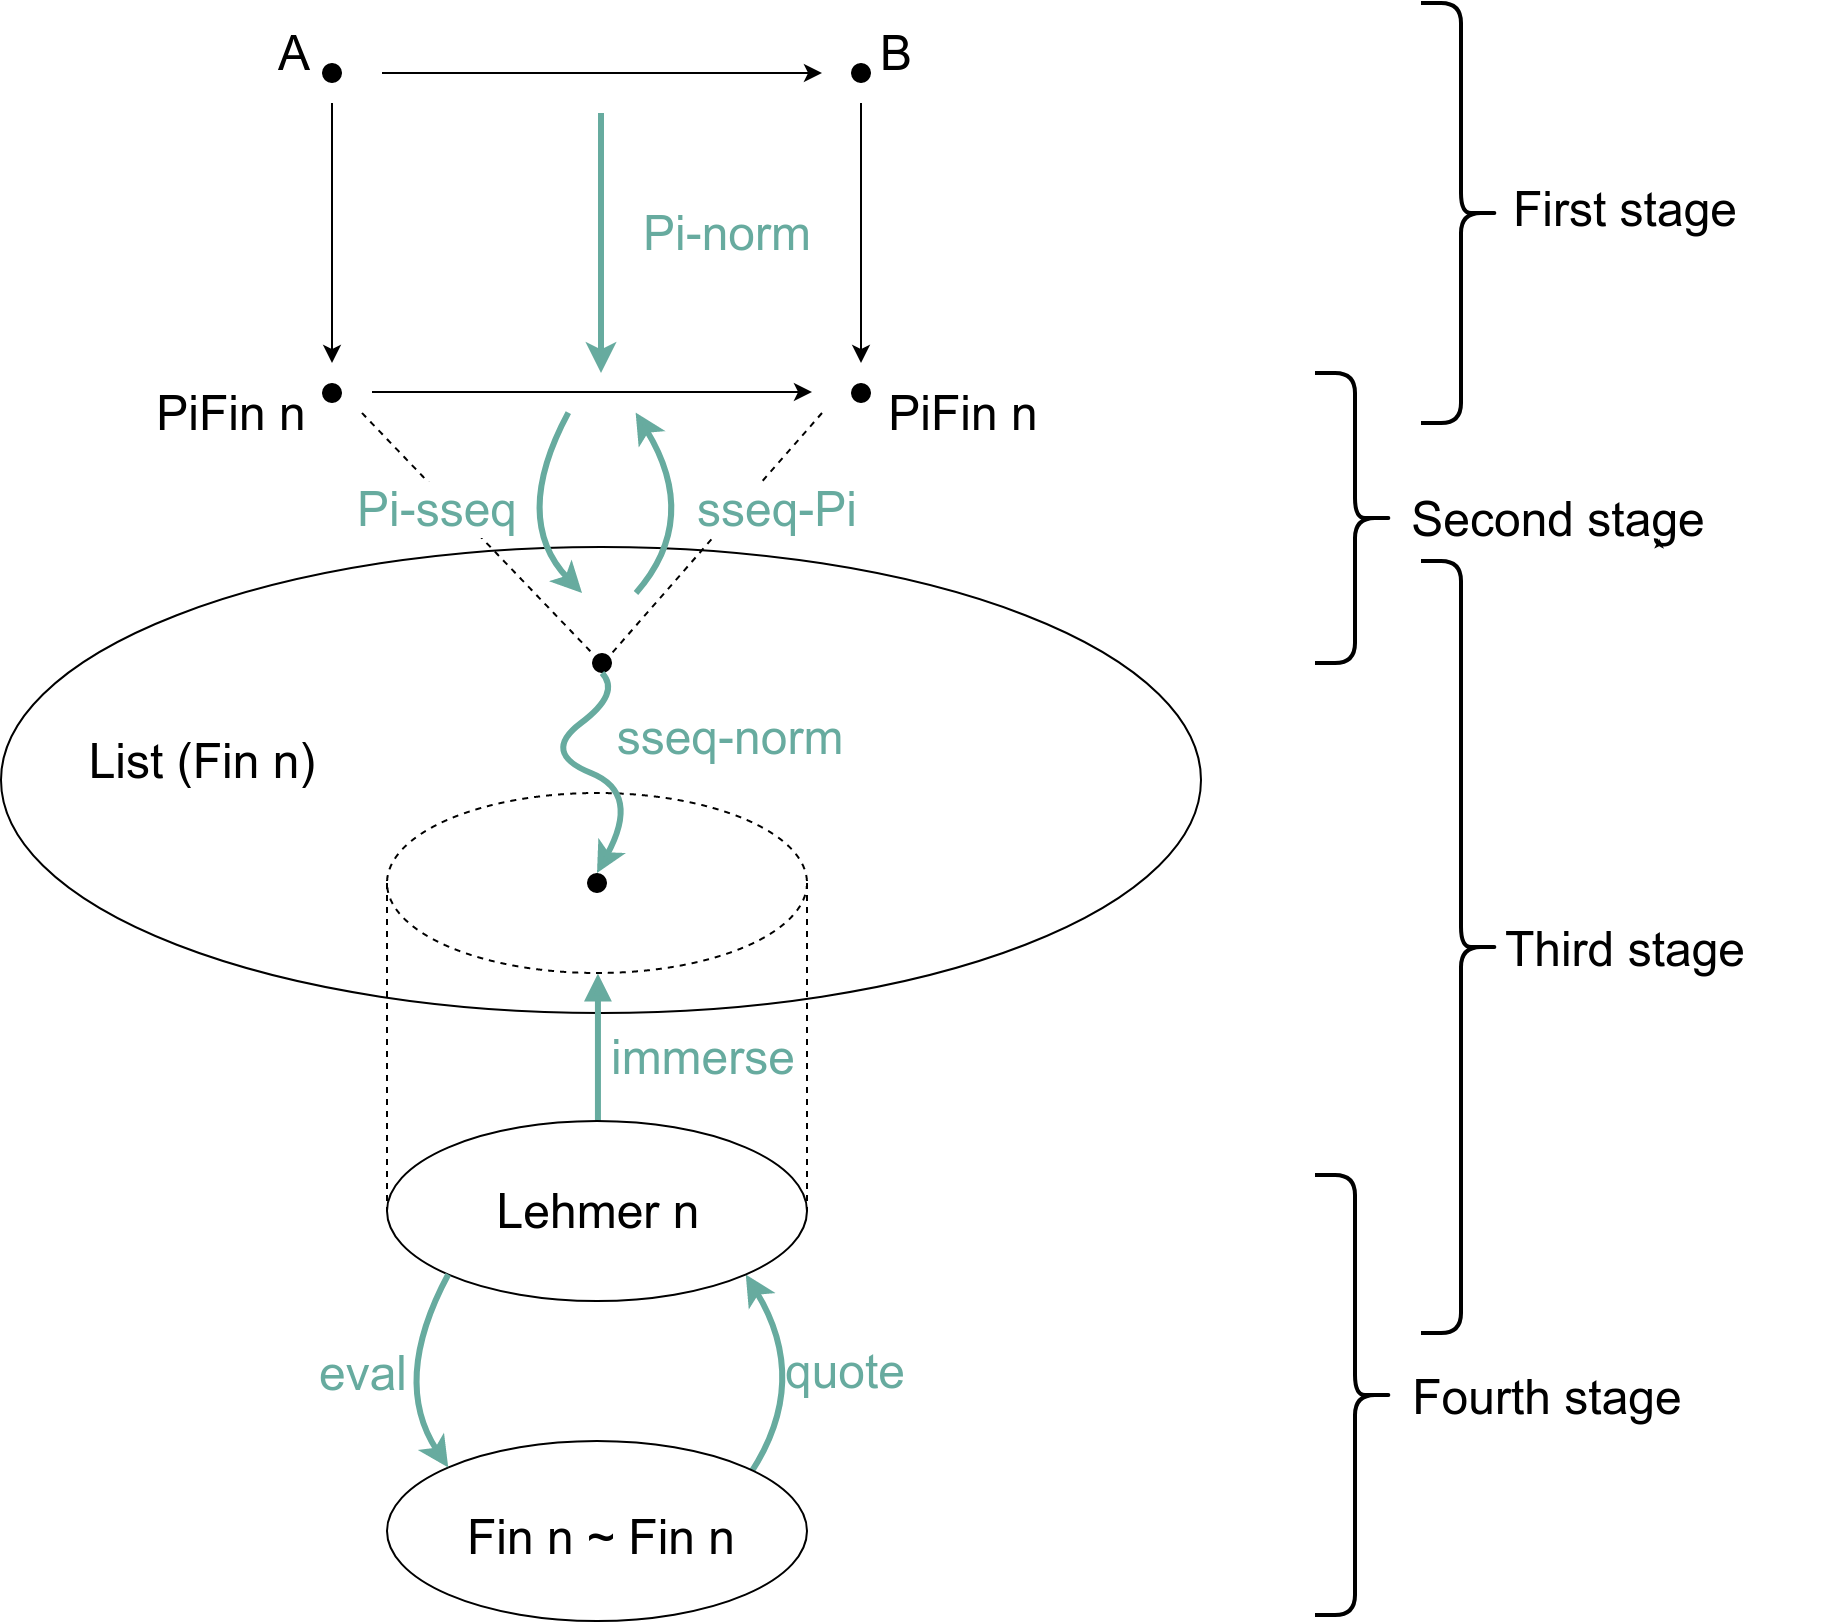
\includegraphics[scale=0.3]{outline.png}
\end{center}

\note{Redo this figure or delete ??}

\note{Spiel about reversible computing and logical reversibility ??}

\note{Spiel about using groupoids for denotational semantics ??}

\note{Could we include a short paragraph about entropy and bits and logical reversibility ??}

\note{Novel interpretation of the univalence axiom, operational and denotational semantics and adequacy.}

-------


% * STLC(first) is the type theory for CCC
%   HoTT is type theory for weak infty groupoids(first)
%   Correspondence between TT and categories are fruitful:
%   answer hard questions about syntax without worrying about presentation
%   normalization of lcal with strong sums: if you have specific syntax; no obvious induction on syntax
%   Lawvere thesis


% * Rig groupoids are interesting! WHY????
%   Add monoidal structure to weak groupoids. Easy. Lists
%   How symmetry is going to act on higher dimension
%   Higher-dim all symmetric; topology higher things abelian groups

% * What is the corresponding type theory ?
%   We give it for the free symmetric groupoid; for other groupoids build on it and add more




%%% Local Variables:
%%% mode: latex
%%% TeX-master: "main"
%%% fill-column: 120
%%% End:

\section{Reversible Programming Languages}~\label{sec:reversible}

\todo{Not the right title.}

\note{This section should explain the main technical parts of the paper
  informally, without using any technology. Use an example, such as, a
  reversible language with $\leq 5$ bits, and examples of permutations and
  transpositions, and when they're equal.}

\note{Motivation: There are two reversible circuits which describe the following permutation. They can be shown to be
  equal using the 2-combinators.}

\[
  \begin{tikzpicture}
    \begin{knot}[clip width=5]
      \filldraw (0,5) circle (2pt) node[above] {0};
      \filldraw (1,5) circle (2pt) node[above] {1};
      \filldraw (2,5) circle (2pt) node[above] {2};
      \filldraw (3,5) circle (2pt) node[above] {3};
      \filldraw (4,5) circle (2pt) node[above] {4};
      \filldraw (0,0) circle (2pt) node[below] {1};
      \filldraw (1,0) circle (2pt) node[below] {4};
      \filldraw (2,0) circle (2pt) node[below] {0};
      \filldraw (3,0) circle (2pt) node[below] {3};
      \filldraw (4,0) circle (2pt) node[below] {2};
      \strand (0,5) .. controls (0.5,0.5) and (1.5,3.5) .. (2,0);
      \strand (1,5) .. controls (0.75,0.5) and (0.25,3.5) .. (0,0);
      \strand (2,5) .. controls (2.5,2.5) and (3.5,1.5) .. (4,0);
      \strand (3,5) .. controls (4.5,2.5) and (4,1.5) .. (3,0);
      \strand (4,5) .. controls (3.5,2.5) and (1.5,2.5) .. (1,0);
      \flipcrossings{4,5};
    \end{knot}
  \end{tikzpicture}
\]

\note{Example: We reduce $\mathsf{swap} : 2 + 2 \leftrightarrow 2 + 2$ to a sequence of adjacent swaps. This is an
  example of a translation from $\PiPlusLang$ to $\PiHatLang$.}

\[
  \begin{tikzpicture}
    \begin{knot}[clip width=4]
      \filldraw (0,4) circle (2pt) node[above] {0};
      \filldraw (1,4) circle (2pt) node[above] {1};
      \filldraw (2,4) circle (2pt) node[above] {2};
      \filldraw (3,4) circle (2pt) node[above] {3};
      \filldraw (0,0) circle (2pt) node[below] {2};
      \filldraw (1,0) circle (2pt) node[below] {3};
      \filldraw (2,0) circle (2pt) node[below] {0};
      \filldraw (3,0) circle (2pt) node[below] {1};
      \strand (0,4) .. controls (0.5,1.5) and (1.5,2.5) .. (2,0);
      \strand (1,4) .. controls (1.5,1.5) and (2.5,2.5) .. (3,0);
      \strand (2,4) .. controls (1.5,1.5) and (1.5,2.5) .. (0,0);
      \strand (3,4) .. controls (2.5,1.5) and (2.5,2.5) .. (1,0);
    \end{knot}
  \end{tikzpicture}
\]

\begin{align*}
  \begin{tikzpicture}
    \begin{knot}[clip width=4]
      \filldraw (0,4) circle (2pt) node[above] {0};
      \filldraw (1,4) circle (2pt) node[above] {1};
      \filldraw (2,4) circle (2pt) node[above] {2};
      \filldraw (3,4) circle (2pt) node[above] {3};
      \filldraw (0,0) circle (2pt) node[below] {0};
      \filldraw (1,0) circle (2pt) node[below] {2};
      \filldraw (2,0) circle (2pt) node[below] {1};
      \filldraw (3,0) circle (2pt) node[below] {3};
      \strand (0,4) to (0,0);
      \strand (1,4) .. controls (0.5,2) and (2.5,2) .. (2,0);
      \strand (2,4) .. controls (2.5,2) and (0.5,2) .. (1,0);
      \strand (3,4) to (3,0);
    \end{knot}
  \end{tikzpicture}
  &&
    \begin{tikzpicture}
      \begin{knot}[clip width=4]
        \filldraw (0,4) circle (2pt) node[above] {0};
        \filldraw (1,4) circle (2pt) node[above] {2};
        \filldraw (2,4) circle (2pt) node[above] {1};
        \filldraw (3,4) circle (2pt) node[above] {3};
        \filldraw (0,0) circle (2pt) node[below] {2};
        \filldraw (1,0) circle (2pt) node[below] {0};
        \filldraw (2,0) circle (2pt) node[below] {1};
        \filldraw (3,0) circle (2pt) node[below] {3};
        \strand (0,4) .. controls (-0.5,2) and (1.5,2) .. (1,0);
        \strand (1,4) .. controls (1.5,2) and (-0.5,2) .. (0,0);
        \strand (2,4) to (2,0);
        \strand (3,4) to (3,0);
      \end{knot}
    \end{tikzpicture}
  \\
  \begin{tikzpicture}
    \begin{knot}[clip width=4]
      \filldraw (0,4) circle (2pt) node[above] {2};
      \filldraw (1,4) circle (2pt) node[above] {0};
      \filldraw (2,4) circle (2pt) node[above] {1};
      \filldraw (3,4) circle (2pt) node[above] {3};
      \filldraw (0,0) circle (2pt) node[below] {2};
      \filldraw (1,0) circle (2pt) node[below] {0};
      \filldraw (2,0) circle (2pt) node[below] {3};
      \filldraw (3,0) circle (2pt) node[below] {1};
      \strand (0,4) to (0,0);
      \strand (1,4) to (1,0);
      \strand (2,4) .. controls (1.5,2) and (3.5,2) .. (3,0);
      \strand (3,4) .. controls (3.5,2) and (1.5,2) .. (2,0);
    \end{knot}
  \end{tikzpicture}
  &&
    \begin{tikzpicture}
      \begin{knot}[clip width=4]
        \filldraw (0,4) circle (2pt) node[above] {2};
        \filldraw (1,4) circle (2pt) node[above] {0};
        \filldraw (2,4) circle (2pt) node[above] {3};
        \filldraw (3,4) circle (2pt) node[above] {1};
        \filldraw (0,0) circle (2pt) node[below] {2};
        \filldraw (1,0) circle (2pt) node[below] {3};
        \filldraw (2,0) circle (2pt) node[below] {0};
        \filldraw (3,0) circle (2pt) node[below] {1};
        \strand (0,4) to (0,0);
        \strand (1,4) .. controls (0.5,2) and (2.5,2) .. (2,0);
        \strand (2,4) .. controls (2.5,2) and (0.5,2) .. (1,0);
        \strand (3,4) to (3,0);
      \end{knot}
    \end{tikzpicture}
\end{align*}

\note{This might be followed by a section which explains the syntax of Pi.}

%%% Local Variables:
%%% mode: latex
%%% TeX-master: "main"
%%% fill-column: 120
%%% End:

\section{Univalent Subuniverses}~\label{sec:univalent}

In this section, we introduce some basic concepts and notation that we use in Homotopy Type Theory. Then, we define
univalent subuniverses and discuss some specific examples.

\subsection{The Type Theory}~\label{subsec:type-theory}

We work in Homotopy Type Theory, in particular, intensional Martin-L\"{o}f Type Theory, with a univalent universe, and
Higher Inductive Types (HITs) for propositional truncations and set quotients. We recall a few basic facts to
familiarise the reader with the notation we use. For more details about basics of HoTT, we refer the reader to the HoTT
book~\cite{univalentfoundationsprogramHomotopyTypeTheory2013}.

\note{It is important that we work in HoTT using it as a metatheory, we care about proof relevance, constructivity, and
  working with higher-dimensional algebraic structures, such as groupoids. Our results are also formalised using general
  tools and principles from HoTT, and computer checked using a proof assistant, using Agda and the HoTT-Agda library.}

\subsubsection{Identity Types}

\vc{I'm explaining everything starting from the categorical language. We do care more about the groupoid structure of
  types, and how to encode groupoids using types, since that's what we use in~\cref{sec:finite}.}

In HoTT, the intensional identity type is the type of paths between two terms of the same type. Given two terms $x:A$
and $y:A$, we write $x \id_{A} y$, or simply $x \id y$, for the equality type between them. In book HoTT, the identity
type is generated by reflexivity $\refl_{x}$, and the eliminator for the identity type is given by path induction or the
$J$-rule. The identity type equips each type with the structure of an infinity groupoid, or a homotopy type.

\todo{Say why it is a groupoid by listing some groupoid laws.}

Functions between types are functors between groupoids. Given a function $f : A \to B$, the functorial action is given
by

\[
  \term{ap}_{f} : \dfun{x,y:A}{x \id_{A} y \to f(x) \id_{B} f(y)}
\]

Type families are functions from a type to the universe, that is, an indexed family of groupoids. The $\term{transport}$
operation gives the functorial action of paths in the indexing type, which is defined by path induction. If
$P : A \to \UU$ is a type family, then for a path $x \id_{A} y$, we have

\[
  \transport{P} : \dfun{x,y:A}{x \id_{A} y \to P(x) \to P(y)}
\]

\todo{Why is the topological viewpoint important, or saying fibrations? Explain the intuition using classifying spaces,
  maybe draw some diagrams.}

From the topological viewpoint, a type family can also be seen as a fibration. For a type family $P : A \to \UU$ and a
point $x : A$, $P(x)$ gives the fiber over $a$. For a path $p : x \id_{A} y$, $\transport{P}{p}$ gives the path lifting
operation. The total space is given by $\dsum{x:A}{P(x)}$ and the first projection ${\pi_1 : \dsum{x:A}{P(x)} \to A}$ to
the base space is the fibration. The lifting operation lifts paths in the base space to paths in the total space. If
$p : x \id_{A} y$ is a path in the base space, and $u : P(x)$, we have

\[
  \term{lift}(u,p) : (x , u) \id_{\dsum{x:A}{P(x)}} (y , \tr{p}{u})
\]

where $\tr{p}{u}$ is shorthand for $\transport{P,p}(u)$.

Further, using the groupoid structure of $A$, we can show that transport lifts paths to equivalences, we define

\[
  \tptEqv{P} : \dfun{x,y:A}{x \id_{A} y \to P(x) \eqv P(y)}
\]

\todo{Explain motivation.}

\begin{definition}[Univalent Fibration]
  $P$ is a univalent type family (or simply a univalent fibration) if $\tptEqv{P}$ is an equivalence.
\end{definition}

\subsubsection{Univalence}

Voevodsky's \emph{univalence} principle characterises paths in the universe. It says that equivalent types are equal, or
the following function is an equivalence.

\[
  \ua : A \id_{\UU} B \to A \eqv B
\]

\todo{Revise.}

Alternatively, one can say that the identity type family $\term{id} : \UU \to \UU$ is univalent.

\subsubsection{Higher Inductive Types}

\todo{Explain homotopy types, $\hProp$, $\hSet$, etc.}

\vc{These are placeholder definitions, need informal explanations and references to the book.}

\begin{definition}[Propositional Truncation]
  Given a type $A$, the propositional truncation $\Trunc[-1]{A}$, or simply $\Trunc{A}$, is a higher inductive type
  generated by the following constructors,
  \begin{itemize}
    \item an inclusion function $\trunc{\blank} : A \to \Trunc{A}$,
    \item for each $x, y : \Trunc{A}$, a path $\term{trunc}(x,y) : x \id_{\Trunc{A}} y$,
  \end{itemize}
  such that, given any type $B$ with
  \begin{itemize}
    \item a function $g : A \to B$,
    \item for each $x, y : B$, a path $\term{trunc*}(x,y) : x \id_{B} y$,
  \end{itemize}
  there is a unique function $f : \Trunc{A} \to B$ such that,
  \begin{itemize}
    \item $f(\trunc{a}) \equiv g(a)$
    \item for each $x, y : \Trunc{A}$, $\ap{f}{\term{trunc}(x,y)} \id_{B} \term{trunc*}(f(x),f(y))$.
  \end{itemize}
\end{definition}

\begin{definition}[Set Quotient]
  Given a type $A$ which is an $\hSet$, and a relation $R : A \to A \to \hProp$, the set-quotient $\quot{A}{R}$ is the
  higher inductive type generated by
  \begin{itemize}
    \item an inclusion function $q : A \to \quot{A}{R}$,
    \item for each $x, y : A$ such that $R(x,y)$, a path $q(x) \id_{\quot{A}{R}} q(y)$,
    \item a set truncation, for each $x, y : \quot{A}{R}$ and $r, s : x \id_{\quot{A}{R}} y$, we have $r \id s$,
  \end{itemize}
  with \review{an appropriate induction principle.}
\end{definition}

We recall that quotients in HoTT are \emph{effective}, that is, if $R$ is an equivalence relation, we have
$R(x,y) \eqv (q(x) \id_{\quot{A}{R}} q(y))$.

\subsection{Univalent Subuniverses}

\todo{Explain motivation. Starting from a univalent universe which classifies all types, we want to define a subuniverse
  which classifies only certain types, for example, types that satisfy some property that we want.}

\begin{definition}[Universe]
  A universe \`{a} la Tarski is given by the following pieces of data,
  \begin{itemize}
    \item a code $U : \UU$,
    \item a decoding function $\El : U \to \UU$.
  \end{itemize}
  If $\El$ is a univalent fibration, $U$ is a univalent universe.
\end{definition}

\begin{definition}[Subuniverse]
  A subtype is a type family $P : \UU \to \UU$ whose fibers are prop-valued, that is, $\forall x, \isProp{P(x)}$. A
  subuniverse generated by a subtype has $U \defeq \dsum{X:\UU}{P(X)}$ and $\El \defeq \fst$.
\end{definition}

\begin{proposition}[Univalent Subuniverse]
  Subuniverses generated by subtypes are univalent.
\end{proposition}

\begin{proof}
  Suppose $(U, \El) \defeq (\dsum{X:\UU}{P(X)}, \fst)$ is a subuniverse generated by a subtype $P : \UU \to \UU$. For
  any $X, Y : \UU$ such that $\phi : P(X)$ and $\psi : P(Y)$, we want to show that
  $\tptEqv{\fst} : (X,\phi) \id (Y,\psi) \to X \eqv Y$ is an equivalence. We construct
  $X \eqv Y \to (X,\phi) \id (Y,\psi)$ by $\ua$ and using the fact that $P(\blank)$ is a proposition. That it is an
  inverse follows by calculation using the appropriate computation rules.
\end{proof}

\begin{example}[$\BAut$]
  The type of self-equivalences on a type $T$ is defined as $\Aut[T] \defeq T \eqv T$, which is an $\infty$-group. The
  subuniverse of types that are merely equal to $T$ is given by $\BAut[T] \defeq \Sub{T}$. This turns out to be the
  classifying space of $\Aut[T]$, as justified by~\cref{lem:loop-deloop}. We write $T_{o} \defeq (T, \trunc{\refl_{T}})$
  for the image of the inclusion of $T$.
\end{example}

\begin{example}
  The univalent subuniverse of types merely equal to $\Bool$ is given by $\BAut[\Bool]$. This can be used to give the
  denotational semantics of a 2-bit reversible language~\cite{caretteReversibleProgramsUnivalent2018}.
\end{example}

\begin{definition}[$\Fin$]
  The type family $\Fin : \Nat \to \UU$ is the type of finite sets indexed by cardinality. It is defined equivalently in
  two different ways,
  \begin{gather*}
    \begin{aligned}
      \Fin[n] & \defeq \dsum{k:\Nat}{k < n}
    \end{aligned}
    \begin{aligned}
      & \Fin[0] \defeq \bot \\
      & \Fin[\suc[n]] \defeq \top \sqcup \Fin[n]
    \end{aligned}
  \end{gather*}
  Note that $\Fin[n]$ is a $\hSet$, and we use the definitions interchangeably.
\end{definition}

\begin{example}
  For any $n : \Nat$, we define the univalent subuniverse of types merely equal to $\Fin[n]$ as $\BAut[\Fin[n]]$. This
  is the universe of finite sets with cardinality equal to $n$. We write $F_{n} \defeq (\Fin[n], \trunc{\refl})$ for the
  image of the inclusion of $\Fin[n]$.
\end{example}

\begin{definition}[$\isFin$]
  We say that a type is finite if it is merely equal to $\Fin[n]$ for some $n$.
  \[
    \isFin[X] \defeq \dsum{n:\Nat}{\SubP{X}{\Fin[n]}}
  \]
  Note that the natural number $n$ need not be truncated, as justified below.
\end{definition}

\begin{proposition}
  For any type $X$, $\isFin[X]$ is a proposition.
\end{proposition}

\begin{proof}
  Suppose we have $(n,\phi) : \isFin[X]$ and $(m,\psi) : \isFin[X]$, we need to show that $(n,\phi) \id (m,\psi)$. It is
  enough to show that $n \id m$. Since $\Nat$ is a set, this is a proposition, so we can use the induction principle of
  propositional truncation to eliminate to $n \id m$, applying it on $\phi$ and $\psi$ respectively. This gives us the
  equalities $X \id \Fin[n]$ and $X \id \Fin[m]$, which gives us $\Fin[n] \id \Fin[m]$, from which $n \id m$ follows by
  applying the first projection.
\end{proof}

\begin{example}
  The univalent subuniverse of \emph{all finite types} is given by
  \[
    \UFin \defeq \dsum{X:\UU}{\isFin[X]}.
  \]
  We write $F_{n} \defeq (\Fin[n], n, \trunc{\refl})$, for the image of the inclusion of $\Fin[n]$. We use this as the
  denotational semantics to interpret our reversible programming language $\PiPlusLang$.
\end{example}

\review{We characterise the path space of univalent subuniverses.}

\begin{proposition}
  If $T$ is an $n$-type, $\BAut[T]$ is an $(n+1)$-type.
\end{proposition}

\begin{proof}
  We need to show that the equality type of $\BAut[T]$ is an $n$-type. Assume $X, Y : \BAut[T]$. Since $\BAut[T]$ is a
  univalent subuniverse, we have $(X \id Y) \eqv (\fst(X) \eqv \fst(Y))$. Note that being an $n$-type is a proposition.
  Since $T$ is an $n$-type, and $\fst(X)$ and $\fst(Y)$ are merely equal to $T$, they're also $n$-types. It follows that
  $\fst(X) \eqv \fst(Y)$ is an $n$-type, and hence $X \id Y$ is an $n$-type.
\end{proof}

\begin{corollary}
  $\UFin$ is a 1-type, that is, a 1-groupoid, or has h-level 3.
\end{corollary}

\begin{lemma}~\label{lem:loop-deloop}
  \[
    \loopspace[\BAut[T],T_{0}] \eqv \Aut[T]
  \]
\end{lemma}

\begin{proof}
  Since $\BAut[T]$ is a univalent universe, it follows that
  \[
    (T_{0} \id_{\BAut[T]} T_{0}) \eqv (\fst(T_{0}) \eqv \fst(T_{0})) \equiv (T \eqv T) \equiv \Aut[T].
  \]
\end{proof}

\begin{corollary}
  For every $n:\Nat$,
  \[
    \loopspace[\UFin[n],F_{n}] \eqv \Aut[\Fin[n]]
  \]
\end{corollary}

%%% Local Variables:
%%% mode: latex
%%% TeX-master: "main"
%%% fill-column: 120
%%% End:

\section{The Group of Permutations}
\label{sec:finite}

% Recap of the previous section
In~\Cref{sec:ufin}, we established that paths in $\UFin$ are equivalent to families of loops on $\Fin[n]$ for every
$n:\Nat$, that is, automorphisms of finite sets of size $n$, with the loopspace encoding the automorphism group.  This
is also known to be the finite symmetric group $\Sn[n]$, making $\UFin$ the \emph{horizontal categorification} of $\Sn$
for every $n$. In this section, we will describe this group syntactically.

% What now?
In order to study syntactic descriptions of permutations, we will hit the problem of deciding whether two descriptions
refer to the same permutation -- in group theory, this is the \emph{word problem} for $\Sn$. Putting it in this form
allows us to connect it to the broader scope of computational group theory and combinatorics -- we can borrow ideas such
as Coxeter relations and Lehmer codes.~\footnote{The concepts we use can be found in any standard textbook on group
theory, or see~\cite{symmetryBook2021} for a univalent point of view.}

% The summary of what we'll do
Thus, the goal of this section is to reconcile two different approaches to defining the symmetric group -- as an
automorphism group, and as a group syntactically presented using \emph{generators} and \emph{relations}. The generators
of the group are similar to the primitive combinators in a (reversible) programming language -- the group structure
gives the composition and inverse operations, and the relations describe how these primitive combinators interact with
each other.

% High-level explanation of technical devices
First, we will define the required notions of free groups and group presentations, and state some of their most
important properties. Then, we introduce our chosen \emph{Coxeter presentation} for $\Sn$. To solve the word problem for
$\Sn$, we will use a rewriting system, with a suitable, well behaved collection of reduction rules corresponding to the
Coxeter presentation equations. Finally, we describe the normal forms in this rewriting system, using Lehmer codes, and prove the
correspondence between them and the type $\Aut[\Fin[n]]$ of automorphisms on a finite set. The generators and relations
we use here will be used to quote back to 1 and 2-combinators in $\PiLang$ (see~\cref{sec:equivalence}).

\subsection{Presenting the permutation group}

One way of thinking about presentations of $\Sn$ is via sorting algorithms, which use different primitive operations. A
sorting algorithm has to calculate a permutation of a list or a finite set, which satisfies the invariant of being a
sorted sequence, which means, the primitive operations of a sorting algorithm are able to generate all the permutations
on a given list. So, a chosen set of reversible operations in a sorting algorithm can be a good candidate for the
generators of a permutation group. For example, we could generate the permutation group on $\Fin[n]$ by using generators
(primitive operations) that:

\begin{itemize}
  \item swap the $i$-th element with the $(i+1)$-th element, that is, adjacent swaps, or
  \item swap the $i$-th element with the $j$-th element, for arbitrary $i$-s and $j$-s, or
  \item swap the $i$-th element with an element at a fixed position, or
  \item reverses a prefix $\Fin[k]$ of $\Fin[n]$ for $k \leq n$, or
  \item cyclically shift any subset of $\Fin[n]$.
\end{itemize}

Bubble sort uses the primitive operation of adjacent swaps, insertion sort and selection sort use the primitive
operation of swapping the $i$-th element with the $j$-th element, cycle sort uses cyclical shifts of subsequences,
pancake sort uses reversals of the prefixes of the list, et cetera. The choice of generators for our presentation is
important for the following reasons.

\begin{itemize}
  \item It affects the difficulty of solving the word problem in $\Sn$ and formalising the proof of its correctness.
  \item The choice of generators dictates which words become normal forms in this presentation of $\Sn$. These normal
        forms dictate the shape of the synthesised and normalised boolean circuits, which is the application we have in
        mind.
  \item Finally, the generators have to closely match the $\PiLang$ combinators so that we can quote back a permutation
        to a $\PiLang$ program, for the proof of completeness.
\end{itemize}

We will show that it is possible to encode all $\PiLang$ combinators using adjacent transpositions
(in~\cref{sec:equivalence}). Group presentations are built by adding equations to a \emph{free group}.

\begin{toappendix}
  \subsection{Groups}
  \label{subsec:groups}

  From universal algebra, a group is simply a set with a 0-ary constant $e$ (the neutral element), a binary operation
  $\blank\mult\blank$ for group multiplication, and a unary inverse operation $\inv{\blank}$. The neutral element has to
  satisfy unit and inverse laws, and the multiplication has to be associative (see~\cref{def:group}).

  A very simple example of a group is $\mathbb{Z}$, where the neutral element is 0, the inverse of $k$ is $-k$, and the
  group multiplication is given by integer addition.

  \begin{definition}[Group]
    \label{def:group}
    In type theory, a group $G$ can be defined as a set $S$ with the following pieces of data:

    \begin{enumerate}
      \item a unit or neutral element $e : S$
      \item a multiplication function $m : S \times S \to S$ written as $(g_{1}, g_{2}) \mapsto g_{1} \mult g_{2}$, that satisfies
            \begin{enumerate}
              \item the unit laws, for all $g : S$, that \( g \mult e \id g \) and \( e \mult g \id g \)
              \item the associativity law, for all $g_{1}, g_{2}, g_{3} : S$, that \( g_{1} \mult (g_{2} \mult g_{3}) \id (g_{1} \mult g_{2}) \mult g_{3} \)
            \end{enumerate}
      \item an inversion function $i : S \to S$ written as $g \mapsto \inv{g}$, that satisfies
            \begin{enumerate}
              \item the inverse laws, for all $g : S$, that \( g \mult \inv{g} \id e \) and \( \inv{g} \mult g \id e \)
            \end{enumerate}
    \end{enumerate}
  \end{definition}
\end{toappendix}

\subsection{Free groups}

Usually, there are are many equations, besides the group axioms, that hold for the elements of a group. For example, in
the group $\Aut[\Bool]$, or $\mathbb{Z}_2$, we have an equation $1 + 1 = 0$, which is not a consequence of the group
axioms, but is specific to this particular group. A free group has the property that no other equations hold except the
ones directly implied by the group axioms. For example, the additive group of integers $\mathbb{Z}$ is the free group on
the singleton set.

\begin{toappendix}
  \begin{definition}[Free group]
    \label{def:free-group}
    Given a set $A$, the free group $F(A)$ on it is given by a higher inductive type with the following point and path
    constructors. Notice the similarity with the definition of a group structure (\cref{def:group}), but note that each
    operation here is a generator for $F(A)$.
    \begin{itemize}
      \item An inclusion function $\eta_{A} : A \to F(A)$
      \item A multiplication function $m : F(A) \times F(A) \to F(A)$
      \item An element $e : F(A)$
      \item An inverse function $i : F(A) \to F(A)$
    \end{itemize}
    \smallskip
    \begin{itemize}
      \item For every $x, y, z : F(A)$, a path $\term{assoc} : m(x, m(y, z)) \id m(m(x, y), z)$
      \item For every $x : F(A)$, paths $\term{unitr} : m(x, e) \id x$ and $\term{unitl} : m(e, x) \id x$
      \item For every $x : F(A)$, paths $\term{invr} : m(x, i(x)) \id e$ and $\term{invl} : m(i(x), x) \id e$
      \item A 0-truncation, for every $x, y : F(A)$ and $p, q : x \id y$, a 2-path $\term{trunc} : p \id q$
    \end{itemize}
  \end{definition}
\end{toappendix}

A group homomorphism between groups $G$ and $H$ is a function $f : G \to H$ between the underlying sets that preserves
the group structure. Giving a group homomorphism out of the free group is equivalent to giving a function out of the
generating set. This is the universal property of free groups, stemming from the free-forgetful adjunction between the
category of groups and sets.

% Informally, it states that if we know how a map $f$ acts on the
% generating set $A$, we know exactly how it acts on every element of the group $F(A)$.

\begin{propositionrep}[Universal Property of $F(A)$]
  \label{prop:free-groups}
  Given a group $G$ and a map $f : A \to G$, there is a unique group homomorphism $\extend{f} : \term{Hom}(F(A), G)$
  such that $\extend{f} \comp \eta_A \htpy f$. Equivalently, composition with $\eta_A$ gives an equivalence
  $\term{Hom}(F(A),G) \eqv A \to G$.
\end{propositionrep}

\begin{toappendix}
  Alternatively, the type of group homomorphisms $h : \term{Hom}(F(A),G)$ satisfying $h \comp \eta_A \htpy f$ is
  contractible.

  % https://q.uiver.app/?q=WzAsMyxbMCwyLCJBIl0sWzAsMCwiRihBKSJdLFsyLDAsIkciXSxbMCwxLCJcXGV0YV9BIl0sWzAsMiwiZiIsMl0sWzEsMiwiXFxleHRlbmR7Zn0iLDAseyJzdHlsZSI6eyJib2R5Ijp7Im5hbWUiOiJkYXNoZWQifX19XSxbMyw0LCJcXGlkIiwwLHsic2hvcnRlbiI6eyJzb3VyY2UiOjIwLCJ0YXJnZXQiOjIwfSwic3R5bGUiOnsiYm9keSI6eyJuYW1lIjoibm9uZSJ9LCJoZWFkIjp7Im5hbWUiOiJub25lIn19fV1d
  \[\begin{tikzcd}
      {F(A)} && G \\
      \\
      A
      \arrow[""{name=0, anchor=center, inner sep=0}, "{\eta_A}", from=3-1, to=1-1]
      \arrow[""{name=1, anchor=center, inner sep=0}, "f"', from=3-1, to=1-3]
      \arrow["{\extend{f}}", dashed, from=1-1, to=1-3]
      \arrow["\id", Rightarrow, draw=none, from=0, to=1]
    \end{tikzcd}\]
\end{toappendix}

Following the universal-algebraic definition, in HoTT, we could use a naive higher inductive type to define the free
group, which enforces the group axioms by adding path constructors (see~\cref{def:free-group}). Using the induction
principle, we can easily verify the universal property. However, since this definition of $F(A)$ has lots of path
constructors corresponding to each group axiom, characterising its path space is difficult.

Instead, we will think about elements of the free group as words over an alphabet of letters drawn from the generating
set \emph{and} the set of their formal inverses. If we take the disjoint union of $A$ with itself, that is, $A + A$ as
the group's underlying set, we can use $\inl/\inr$ to mark the elements -- $\inl{a}$ means $a$ and $\inr{a}$ means
$\inv{a}$. Then, we can encode the free group using the free monoid, that is, lists of $A + A$. Additionally, we need to
ensure that the inverse laws hold, so we have to coalesce adjacent occurences of $a$ and $\inv{a}$.

\begin{definition}[Free group]
  Let $A$ be a set, and $\List[\blank]$ the free monoid. The free group $F(A)$ on $A$ is the set-quotient of $\List[A +
      A]$ by the congruence closure of the relation $a \cons \inv{a} \cons \nil \sim \nil$ and $\inv{a} \cons a \cons \nil
    \sim \nil$.
\end{definition}

\begin{proposition}
  $F(A) \defeq \quot{\List[A + A]}{\sim^{\ast}}$ has a group structure, with the empty list $\nil$ for the neutral
  element, multiplication given by list append $\append$, and inverse given by flipping $\inl$ and $\inr$, followed by
  reversing the list. Further, $F(A)$ with $\eta_A(a) \defeq \inl(a) \cons \nil$ satisfies the universal property of
  free groups, as stated in~\Cref{prop:free-groups}.
\end{proposition}

\subsection{Group presentations}

A presentation of a group builds it by starting from the free group $F(A)$ and introducing additional equations that are
satisfied in the resulting group. For example, if we take $F(\unit) \defeq \mathbb{Z}$ and add an equation $1 + 1 = 0$,
the resulting group would be $\mathbb{Z}_2 \eqv \Aut[\Bool]$. Note that not all groups have finite (or computable)
presentations, and, a group can have any number of different presentations.

\begin{definition}[Group presentation]
  \label{def:presentation}
  Let $A$ be a set and $R : \List[A + A] \to \List[A + A] \to \UU$ a binary relation on $\List[A + A]$. The group
  $F(\langle A ; R \rangle)$ presented by $A$ and $R$, is given by the set-quotient of the free group $F(A)$ by the
  congruence closure of $R$.
\end{definition}

The universal property of the above definition is similar to~\Cref{prop:free-groups} except the relation has to be
preserved by the function mapping out of the generating set.

\begin{proposition}[Universal property of $F(\langle A ; R \rangle)$]
  Given a group $G$ and a map $f : A \to G$, such that $f$ extended to $F(A)$ respects $R$, there is a unique group
  homomorphism $\extend{f} : \term{Hom}(F(\langle A ; R \rangle), G)$ such that $\extend{f} \comp \eta_A \htpy f$.
\end{proposition}

Before, the only way to decide the equality of two elements in a group was to evaluate and check them on the nose, but
in a group presentation, this is reduced to deciding whether one word -- a representative of the equivalence class of
the group's elements, can be reduced to another word, using the group's relations. However, these equations are not
directed, so it is not always possible to construct a well-behaved rewriting system. In general, the word problem for
groups is undecidable.

\paragraph{Coxeter Presentation} To present the group $\Sn$, the primitive operations we use will be adjacent swaps.
When dealing with permutations on an $n + 1$-element set, there are $n$ adjacent transpositions -- transposition number
$k$ swaps elements at indices $k$ and $k+1$. Thus, the generating set is $\Fin[n]$. There are three relations that we're
going to specify for this presentation -- we visualise them as braid diagrams in~\Cref{fig:coxeter-braid}.

\begin{enumerate}[leftmargin=*]
  \item[\labelcref{fig:coxeter-a}] Swapping the same two elements twice in a row should be the same as doing nothing.
  \item[\labelcref{fig:coxeter-b}] When swapping two distinct pairs of elements, the order in which swapping happens
        should not matter, that is, we can slide the wires freely.
  \item[\labelcref{fig:coxeter-c}] There are two equivalent ways of swapping the first and last elements in a sequence
        of three elements.
\end{enumerate}

\begin{figure}
  \centering
  \begin{subfigure}[b]{0.25\textwidth}
    \centering
    \begin{tikzpicture}
      \pic[local bounding box=my braid,braid/.cd,
        number of strands = 2,
        width = 0.4cm,
        height = 0.4cm,
        border height = 0.3cm,
        thick] at (0, 0)
      {braid={ s_1, s_1}};
      \node[font=\large] at (1, 0.7) {\(=\)};
      \pic[local bounding box=my braid,braid/.cd,
        number of strands = 2,
        width = 0.4cm,
        height = 0.4cm,
        border height = 0.3cm,
        thick] at (1.6, 0)
      {braid={ 1, 1}};
    \end{tikzpicture}
    \caption{$\cancel$}
    \label{fig:coxeter-a}
  \end{subfigure}
  \begin{subfigure}[b]{0.4\textwidth}
    \centering
    \begin{tikzpicture}
      \pic[local bounding box=my braid,braid/.cd,
        number of strands = 2,
        width = 0.4cm,
        height = 0.4cm,
        border height = 0.3cm,
        thick] at (0, 0)
      {braid={ s_1, 1}};
      \node[] at (0.7, 0.7) {\(\dots\)};
      \pic[local bounding box=my braid,braid/.cd,
        number of strands = 2,
        width = 0.4cm,
        height = 0.4cm,
        border height = 0.3cm,
        thick] at (1, 0)
      {braid={ 1, s_1 }};
      \node[font=\large] at (1.9, 0.7) {\(=\)};
      \pic[local bounding box=my braid,braid/.cd,
        number of strands = 2,
        width = 0.4cm,
        height = 0.4cm,
        border height = 0.3cm,
        thick] at (2.4, 0)
      {braid={ 1, s_1}};
      \node[] at (3.1, 0.7) {\(\dots\)};
      \pic[local bounding box=my braid,braid/.cd,
        number of strands = 2,
        width = 0.4cm,
        height = 0.4cm,
        border height = 0.3cm,
        thick] at (3.4, 0)
      {braid={ s_1, 1}};
    \end{tikzpicture}
    \caption{$\swap$}
    \label{fig:coxeter-b}
  \end{subfigure}
  \begin{subfigure}[b]{0.25\textwidth}
    \centering
    \begin{tikzpicture}
      \pic[local bounding box=my braid,braid/.cd,
        number of strands = 3,
        width = 0.4cm,
        height = 0.4cm,
        border height = 0.1cm,
        thick] at (0, 0)
      {braid={ s_2, s_1, s_2}};
      \node[font=\large] at (1.4, 0.7) {\(=\)};
      \pic[local bounding box=my braid,braid/.cd,
        number of strands = 3,
        width = 0.4cm,
        height = 0.4cm,
        border height = 0.1cm,
        thick] at (2, 0)
      {braid={ s_1, s_2, s_1}};
    \end{tikzpicture}
    \caption{$\braid$}
    \label{fig:coxeter-c}
  \end{subfigure}
  \caption{Braiding diarams for Coxeter relations.}
  \label{fig:coxeter-braid}
\end{figure}

This construction is called a Coxeter presentation of $\Sn$. Writing it formally, we encode the rules discussed above
using a relation $\cox$ on $\List[\Fin[n]]$ (\cref{def:cox}), and then take its congruence closure $\cox*$
(\cref{def:coxstar}).

\begin{definition}[$\cox : {\List[\Fin[n]]} \to {\List[\Fin[n]]} \to {\UU}$]
  \label{def:cox}
  \begin{align*}
    \cancel
     & : \forall n \to (n \cons n \cons \nil) \cox \nil                                                     \\
    \swap
     & : \forall k, n \to (\suc[k] < n) \to (n \cons k \cons \nil) \cox (k \cons n \cons \nil)              \\
    \braid
     & : \forall n \to (\suc[n] \cons n \cons \suc[n] \cons \nil) \cox (n \cons \suc[n] \cons n \cons \nil)
  \end{align*}
\end{definition}

\begin{toappendix}
  \begin{definition}[$\cox* : {\List[\Fin[n]]} \to {\List[\Fin[n]]} \to {\UU}$]
    \label{def:coxstar}
    \begin{align*}
      \reflr{\cox}
       & : \forall w \to w \cox* w                                                                                                           \\
      \symr{\cox}
       & : \forall w_{1}, w_{2} \to w_{1} \cox* w_{2} \to w_{2} \cox* w_{1}                                                                  \\
      \transr{\cox}
       & : \forall w_{1}, w_{2}, w_{3} \to  w_{1} \cox* w_{2} \to w_{2} \cox* w_{3} \to w_{1} \cox* w_{3}                                    \\
      \congrf{\cox}{\append}
       & : \forall w_{1}, w_{2}, w_{3}, w_{4} \to  w_{1} \cox* w_{2} \to w_{3} \cox* w_{4} \to w_{1} \append w_{3} \cox* w_{2} \append w_{4} \\
      \relr{\cox}
       & : \forall w_{1}, w_{2} \to w_{1} \cox w_{2} \to w_{1} \cox* w_{2}
    \end{align*}
  \end{definition}
\end{toappendix}

The idea for solving the word problem for $\Sn$ is to turn these undirected relations into a rewriting
system $(\List[\Fin[n]],\cox*)$, so that, by repeatedly applying the reduction rules as long as possible, any two
$\cox*$-equal terms would eventually converge to the same normal form.

For this to work, we first need the system to have the termination property, meaning that there are no infinite
reductions. We observe that after throwing out reflexivity and symmetry, the right hand sides of the relations $\cox*$
are strictly smaller than the left hand sides, in terms of the lexicographical ordering on words in $\Fin[n]$ (which is
well-founded). Thus, by directing the relation from left to right, we would get the termination property out of the box.
Second, we need the normal forms to be unique, so that we can get a normalisation function. This will be true if the
rewriting system is confluent -- meaning that all critical pairs, that is, terms with overlapping possible reduction
rules, have to converge. For example, in our system, the pair in~\Cref{fig:critical-pairs-converging} converges.
Unfortunately, this is not true for all critical pairs -- an  example is in~\Cref{fig:critical-pairs-non-converging},
where left and right endpoints are normal with respect to the $\cox*$ relation.

% \begin{figure}
% \[
%   \begin{array}{lcr}
%     \gspan[\braid][\braid]{\tau_2\tau_1\tau_2\tau_1\tau_2}{\tau_1\tau_2\tau_1\tau_1\tau_2}{\tau_2\tau_1\tau_1\tau_2\tau_1}
%      &
%     \text{or}
%      &
%     \gspan[\braid][\cancel]{\tau_2\tau_1\tau_2\tau_2}{\tau_1\tau_2\tau_1\tau_2}{\tau_2\tau_1}
%   \end{array}
% \]
% \caption{Critical pairs}
% \label{fig:critical-pairs}
% \end{figure}
%  \begin{subfigure}[]{0.45\textwidth}
%    % https://q.uiver.app/?q=WzAsNSxbMiwwLCJcXHRhdV8yXFx0YXVfMVxcdGF1XzJcXHRhdV8yIl0sWzAsMSwiXFx0YXVfMVxcdGF1XzJcXHRhdV8xXFx0YXVfMiJdLFsyLDQsIlxcdGF1XzJcXHRhdV8xIl0sWzAsMiwiXFx0YXVfMVxcdGF1XzJcXHRhdV8xXFx0YXVfMiJdLFsxLDMsIlxcdGF1XzFcXHRhdV8xXFx0YXVfMlxcdGF1XzEiXSxbMCwxLCJicmFpZCIsMix7InN0eWxlIjp7ImJvZHkiOnsibmFtZSI6InNxdWlnZ2x5In19fV0sWzAsMiwiY2FuY2VsIiwwLHsic3R5bGUiOnsiYm9keSI6eyJuYW1lIjoic3F1aWdnbHkifX19XSxbMSwzLCJicmFpZCIsMix7InN0eWxlIjp7ImJvZHkiOnsibmFtZSI6InNxdWlnZ2x5In19fV0sWzMsNCwiYnJhaWQiLDIseyJzdHlsZSI6eyJib2R5Ijp7Im5hbWUiOiJzcXVpZ2dseSJ9fX1dLFs0LDIsImNhbmNlbCIsMix7InN0eWxlIjp7ImJvZHkiOnsibmFtZSI6InNxdWlnZ2x5In19fV1d
%    \adjustbox{scale=\scalef,center}{
%      \begin{tikzcd}
%        && {\tau_2\tau_1\tau_2\tau_2} \\
%        {\tau_1\tau_2\tau_1\tau_2} \\
%        {\tau_1\tau_2\tau_1\tau_2} \\
%        & {\tau_1\tau_1\tau_2\tau_1} \\
%        && {\tau_2\tau_1}
%        \arrow["\braid"', squiggly, from=1-3, to=2-1]
%        \arrow["\cancel", squiggly, from=1-3, to=5-3]
%        \arrow["\braid"', squiggly, from=2-1, to=3-1]
%        \arrow["\braid"', squiggly, from=3-1, to=4-2]
%        \arrow["\cancel"', squiggly, from=4-2, to=5-3]
%      \end{tikzcd}
%    }
%  \end{subfigure}
%   \begin{subfigure}[]{0.45\textwidth}
%    $\gspan[\braid][\swap]{\tau_3\tau_2\tau_3\tau_1}{\tau_2\tau_3\tau_2\tau_1}{\tau_3\tau_2\tau_1\tau_3}$
%    \caption{Non-converging critical pairs}
%    \label{fig:critical-pairs-non-converging}
%  \end{subfigure}

% a + \UOLoverbrace{b +}[c + d]ˆx \UOLunderbrace{+ e}_y + f

\begin{figure}
  \centering
  \begin{subfigure}[b]{0.35\textwidth}
    % https://q.uiver.app/?q=WzAsNixbMSwwLCJcXHRhdV8yXFx0YXVfMVxcdGF1XzJcXHRhdV8xXFx0YXVfMiJdLFswLDEsIlxcdGF1XzFcXHRhdV8yXFx0YXVfMVxcdGF1XzFcXHRhdV8yIl0sWzIsMSwiXFx0YXVfMlxcdGF1XzFcXHRhdV8xXFx0YXVfMlxcdGF1XzEiXSxbMCwyLCJcXHRhdV8xXFx0YXVfMlxcdGF1XzIiXSxbMSwzLCJcXHRhdV8xIl0sWzIsMiwiXFx0YXVfMlxcdGF1XzJcXHRhdV8xIl0sWzAsMSwiYnJhaWQiLDIseyJzdHlsZSI6eyJib2R5Ijp7Im5hbWUiOiJzcXVpZ2dseSJ9fX1dLFswLDIsImJyYWlkIiwwLHsic3R5bGUiOnsiYm9keSI6eyJuYW1lIjoic3F1aWdnbHkifX19XSxbMSwzLCJjYW5jZWwiLDIseyJzdHlsZSI6eyJib2R5Ijp7Im5hbWUiOiJzcXVpZ2dseSJ9fX1dLFszLDQsImNhbmNlbCIsMix7InN0eWxlIjp7ImJvZHkiOnsibmFtZSI6InNxdWlnZ2x5In19fV0sWzIsNSwiY2FuY2VsIiwwLHsic3R5bGUiOnsiYm9keSI6eyJuYW1lIjoic3F1aWdnbHkifX19XSxbNSw0LCJjYW5jZWwiLDAseyJzdHlsZSI6eyJib2R5Ijp7Im5hbWUiOiJzcXVpZ2dseSJ9fX1dXQ==
    \adjustbox{scale=\scalef,center}{
      \begin{tikzcd}
        & {\UOLoverline{\tau_2\tau_1}[\tau_2]\UOLunderline{\tau_1\tau_2}} \\
        {\tau_1\tau_2\overline{\tau_1\tau_1}\tau_2} && {\tau_2\underline{\tau_1\tau_1}\tau_2\tau_1} \\
        {\tau_1\overline{\tau_2\tau_2}} && {\underline{\tau_2\tau_2}\tau_1} \\
        & {\tau_1}
        \arrow["\braid"', squiggly, from=1-2, to=2-1]
        \arrow["\braid", squiggly, from=1-2, to=2-3]
        \arrow["\cancel"', squiggly, from=2-1, to=3-1]
        \arrow["\cancel"', squiggly, from=3-1, to=4-2]
        \arrow["\cancel", squiggly, from=2-3, to=3-3]
        \arrow["\cancel", squiggly, from=3-3, to=4-2]
      \end{tikzcd}
    }
    \caption{Converging critical pair}
    \label{fig:critical-pairs-converging}
  \end{subfigure}
  \begin{subfigure}[b]{0.55\textwidth}
    \adjustbox{scale=\scalef,center}{
      % https://q.uiver.app/?q=WzAsMyxbMSwwLCJcXHRhdV8zXFx0YXVfMlxcdGF1XzNcXHRhdV8xIl0sWzAsMiwiXFx0YXVfMlxcdGF1XzNcXHRhdV8yXFx0YXVfMSJdLFszLDEsIlxcdGF1XzNcXHRhdV8yXFx0YXVfMVxcdGF1XzMiXSxbMCwxLCJicmFpZCIsMix7InN0eWxlIjp7ImJvZHkiOnsibmFtZSI6InNxdWlnZ2x5In19fV0sWzAsMiwiYnJhaWQiLDAseyJzdHlsZSI6eyJib2R5Ijp7Im5hbWUiOiJzcXVpZ2dseSJ9fX1dLFsyLDEsIlxcbG9uZ2JyYWlkIiwwLHsic3R5bGUiOnsiYm9keSI6eyJuYW1lIjoic3F1aWdnbHkifX19XV0=
      \begin{tikzcd}
        & {\UOLoverline{\tau_3\tau_2}[\tau_3]\UOLunderline{\tau_1}} \\
        &&& {\underline{\tau_3\tau_2\tau_1\tau_3}} \\
        {\tau_2\tau_3\tau_2\tau_1}
        \arrow["\braid"', squiggly, from=1-2, to=3-1]
        \arrow["\swap", squiggly, from=1-2, to=2-4]
        \arrow["\longbraid", squiggly, from=2-4, to=3-1]
      \end{tikzcd}
    }
    \caption{Non-converging critical pair that converges with $\longbraid$}
    \label{fig:critical-pairs-non-converging}
  \end{subfigure}

  \caption{Critical Pairs in $\cox*$}
  \label{fig:critical-pairs}
\end{figure}

\subsection{Rewriting via Coxeter}

Because of this counter-example, the relations have to be changed. In this section, we formally define a rewriting
system $(\List[\Fin[n]], \longcox)$, partially based on the Coxeter relations, and prove that it has the desired
properties of confluence and termination. We prove that the new relation defined by this system is equivalent, in a
technical sense, to the standard Coxeter relation $\cox*$. First, we need to define a function $n \downf k$.

\begin{definition}[$\downf : (n : \Nat) \to (k : \Nat) \to {\List[\Fin[k + n]]}$]
  \begin{align*}
    n \downf \zero   & \defeq \nil                       \\
    n \downf \suc[k] & \defeq (k + n) \cons (n \downf k)
  \end{align*}
\end{definition}

\noindent The result of this function is the sequence \([k + n - 1, k + n - 2, k + n - 3, \ldots, n]\), which is a
sequence of transpositions that moves the element at index $k + n$ left by $k$ places, shifting all the elements in
between one place right (see~\cref{fig:downf}). Then, the directed relation $\longcox$ is defined with the following
generators (inlining the congruence closure in $\longcox$, allowing arbitrary reductions inside the list).

\begin{definition}[$\longcox : {\List[\Fin[n]]} \to {\List[\Fin[n]]} \to {\UU}$]
  \begin{align*}
    \longcancel
     & : \forall n, l, r \to (l \append n \cons n \cons r) \longcox (l \append r)                                                                      \\
    \longswap
     & : \forall n, k, l, r \to (\suc[k] < n) \to (l \append n \cons k \cons r) \longcox (l \append k \cons n \append r)                               \\
    \longbraid
     & : \forall n, k, l, r \to (l \append (n \downf 2 + k) \append (1 + k + n) \cons r) \longcox (l \append (k + n) \cons (n \downf 2 + k) \append r)
  \end{align*}
\end{definition}

\noindent Constructors $\longcancel$ and $\longswap$ correspond directly to the appropriate constructors of $\cox$ and
can be visualised in the same way as before. The remaining constructor $\longbraid$ uses the $\downf$ function to
exchange the order of a long sequence of transpositions and a single transposition afterwards. For example, for $n = 0$
and $k = 3$, it allows for the reduction $[4, 3, 2, 1, 0, 4] \longcox [3, 4, 3, 2, 1, 0]$ (see~\cref{fig:longcox} --
note the distinction between wires, where numbers represent the values, and transpositions, where numbers represent
which wires are crossing).

\begin{figure}
  \begin{subfigure}[b]{0.3\textwidth}
    \centering
    \begin{tikzpicture}
      \def\nstrandsdf{7}
      \pic[local bounding box=my braid,braid/.cd,
        number of strands = \nstrandsdf,
        width = 0.4cm,
        height = 0.4cm,
        border height = 0.1cm,
        thick,
        name prefix=braid]
      {braid={s_1, s_2, s_3, s_4, s_5, s_6}};
      % \draw[thick] % draws the top/bottom bars
      % ([xshift=-1ex]my braid.north west) --  ([xshift=1ex]my braid.north east)
      % ([xshift=-1ex]my braid.south west) --  ([xshift=1ex]my braid.south east);
      \foreach \n in {1,...,\nstrandsdf}{
          \pgfmathtruncatemacro{\nminusone}{\n - 1}
          \node at (braid-\n-s)[yshift = 2.8cm] {\nminusone};
        }
      % labels the bottom bar
      \node at (braid-1-e)[yshift = -2.8cm] {5};
      \node at (braid-2-e)[yshift = -2.8cm] {6};
      \node at (braid-3-e)[yshift = -2.8cm] {0};
      \node at (braid-4-e)[yshift = -2.8cm] {1};
      \node at (braid-5-e)[yshift = -2.8cm] {2};
      \node at (braid-6-e)[yshift = -2.8cm] {3};
      \node at (braid-7-e)[yshift = -2.8cm] {4};
    \end{tikzpicture}
    \caption{$0 \downf 6$}
    \label{fig:downf}
  \end{subfigure}
  \hfill
  \begin{subfigure}[b]{0.6\textwidth}
    \centering
    \begin{tikzpicture}
      \def\nstrandsbl{6}
      \pic[local bounding box=my braid,braid/.cd,
        number of strands = \nstrandsbl, % number of  strands
        width = 0.4cm,
        height = 0.4cm,
        border height = 0.1cm,
        thick,
        name prefix=braid] at (0, 0)
      {braid={s_5, s_1, s_2, s_3, s_4, s_5}};
      \node[font=\large] at (3, 1.3) {\(\rightarrow\)};
      % \draw[thick] % draws the top/bottom bars
      % ([xshift=-1ex]my braid.north west) --  ([xshift=1ex]my braid.north east)
      % ([xshift=-1ex]my braid.south west) --  ([xshift=1ex]my braid.south east);
      \foreach \n in {1,...,\nstrandsbl}{
          \pgfmathtruncatemacro{\nminusone}{\n - 1}
          \node at (braid-\n-s)[yshift = 2.8cm] {\nminusone};
        }
      % labels the bottom bar
      \node at (braid-1-e)[yshift = -2.8cm] {3};
      \node at (braid-2-e)[yshift = -2.8cm] {5};
      \node at (braid-3-e)[yshift = -2.8cm] {0};
      \node at (braid-4-e)[yshift = -2.8cm] {1};
      \node at (braid-5-e)[yshift = -2.8cm] {4};
      \node at (braid-6-e)[yshift = -2.8cm] {2};

      \def\nstrandsbr{6}
      \pic[local bounding box=my braid,braid/.cd,
        number of strands = \nstrandsbr,
        width = 0.4cm,
        height = 0.4cm,
        border height = 0.1cm,
        thick,
        name prefix=braid] at (4, 0)
      {braid={s_1, s_2, s_3, s_4, s_5, s_4}};
      % \draw[thick] % draws the top/bottom bars
      % ([xshift=-1ex]my braid.north west) --  ([xshift=1ex]my braid.north east)
      % ([xshift=-1ex]my braid.south west) --  ([xshift=1ex]my braid.south east);
      \foreach \n in {1,...,\nstrandsbl}{
          \pgfmathtruncatemacro{\nminusone}{\n - 1}
          \node at (braid-\n-s)[yshift = 2.8cm] {\nminusone};
        }
      % labels the bottom bar
      \node at (braid-1-e)[yshift = -2.8cm] {3};
      \node at (braid-2-e)[yshift = -2.8cm] {5};
      \node at (braid-3-e)[yshift = -2.8cm] {0};
      \node at (braid-4-e)[yshift = -2.8cm] {1};
      \node at (braid-5-e)[yshift = -2.8cm] {4};
      \node at (braid-6-e)[yshift = -2.8cm] {2};
    \end{tikzpicture}
    \caption{ $\longbraid$ with $n = 0$ and $k = 3$}
    \label{fig:longcox}
  \end{subfigure}
  \caption{Braiding diagrams for modified Coxeter relations.}
  \label{fig:coxeter-braid-mod}
\end{figure}
% in terms of the lexicographic order on $\List[\Fin[n]]$.

\begin{toappendix}
  \begin{definition}[$\longcoxstar : {\List[\Fin[n]]} \to {\List[\Fin[n]]} \to {\UU}$]
    \label{def:longcox-star}
    \begin{align*}
      \reflr{\longcox}
       & : \forall w \to w \longcoxstar w                                                                                  \\
      \transr{\longcox}
       & : \forall w_{1}, w_{2}, w_{3} \to  w_{1} \longcox w_{2} \to w_{2} \longcoxstar w_{3} \to w_{1} \longcoxstar w_{3}
    \end{align*}
  \end{definition}

  \begin{definition}[$\longcoxplus : {\List[\Fin[n]]} \to {\List[\Fin[n]]} \to {\UU}$]
    \label{def:longcox-plus}
    \begin{align*}
      \relr{\longcoxplus}
       & : \forall w_{1}, w_{2} \to w_{1} \longcox w_{2} \to w_{1} \longcoxplus w_{2}                                      \\
      \transr{\longcoxplus}
       & : \forall w_{1}, w_{2}, w_{3} \to  w_{1} \longcox w_{2} \to w_{2} \longcoxplus w_{3} \to w_{1} \longcoxplus w_{3}
    \end{align*}
  \end{definition}
\end{toappendix}

Note that the previous $\braid$ rule is a special case of $\longbraid$, with $k = 0$. As before, the left-hand sides of
the relation are (lexicographically) strictly larger than the right-hand sides. We define the transitive closure of
$\longcox$ to be $\longcoxplus$ (\cref{def:longcox-plus}) and its reflexive-transitive closure to be $\longcoxstar$
(\cref{def:longcox-star}).

Despite the increased complexity of the generators, the rewriting system $(\List[\Fin[n]],\longcox)$ has the properties
we desire. It satisfies local confluence, that is, the Church-Rosser (diamond) property -- for example, using
$\longbraid$, we can now show the problematic critical pair \cref{fig:critical-pairs-non-converging} converges, and, it
is terminating, so by Newman's lemma, it produces a unique normal form. We follow the terminology
of~\citet*{huetConfluentReductionsAbstract1980a,krausCoherenceWellFoundednessTaming2020} to state our results formally.

\begin{theorem}
  \label{prop:nf}
  \leavevmode
  \begin{enumerate}
    \item $\longcox$ is (locally) confluent. For every span $\coxspan{w_{1}}{w_{2}}{w_{3}}$, there is a matching
          extended cospan $\coxcospan*{w_{2}}{w_{3}}{w}$.
    \item $\longcoxplus$ is terminating. For every $w \longcoxplus v$, it holds that $v < w$, where $<$ is the (well-founded)
          lexicographic ordering on $\List[\Fin[n]]$.
    \item $\longcoxstar$ is confluent. For every extended span $\coxspan*{w_{1}}{w_{2}}{w_{3}}$, there is a matching
          extended cospan $\coxcospan*{w_{2}}{w_{3}}{w}$.
    \item For every $w$, there exists a unique normal form $v$ such that $w \longcoxstar v$.~\label{prop:nf-uniqueness}
  \end{enumerate}
\end{theorem}

The modified form of the Coxeter relations are unwieldy and difficult to prove properties about by induction. However,
we can make the following observation relating it to $\cox*$.

\begin{proposition}
  \label{prop:coxlongcox}
  The relations $\cox*$ and $\longcoxstar$ are equivalent in the following sense: for every $w$ and $v$, $w \cox* v$ iff
  there is a $u$ such that $\coxcospan*{w}{v}{u}$.
\end{proposition}

By~\Cref{prop:nf}~\ref{prop:nf-uniqueness}, we get a unique choice function $\normf : {\List[\Fin[n]]} \to
  {\List[\Fin[n]]}$ that produces a normal form for terms of $\List[\Fin[n]]$. We state two important properties enjoyed
by $\normf$.

\begin{proposition}
  \leavevmode
  \begin{enumerate}
    \item For all $l : \List[\Fin[n]]$, we have that $l \cox* \normf(l)$.
    \item $\normf$ is idempotent, that is, $\normf \comp \normf \htpy \normf$.
  \end{enumerate}
\end{proposition}

\noindent Finally, we define the type $\Sn$ as the set-quotient of $\List[\Fin[n]]$ by $\cox*$,

\begin{definition}[$\Sn$]
  \(\Sn \defeq \quot{\List(\Fin[n])}{\cox*}\)
\end{definition}

\noindent Note that reductions need not be unique, hence $w \cox* v$ is not necessarily a proposition. So, the quotient
$\Sn$ is not effective, that is, $\quotrel : w \cox* v \to q(w) \id q(v)$ is not an equivalence. Using the $\normf$
function, we could instead define a new relation $\approx$ to equate those terms that have the same normal form, $(w
  \approx v) \defeq (\normf(w) \id \normf(v))$. This relation is prop-valued, and we could quotient $\List[\Fin[n]]$ by
$\approx$, obtaining an equivalent definition for $\Sn$.

\begin{proposition}
  \leavevmode
  \begin{enumerate}
    \item $\normf$ splits into a section-retraction pair, that is, we have ${\List[\Fin[n]]} \xrightarrow{s} \Sn[n]
            \xrightarrow{r} {\List[\Fin[n]]}$ such that $s \comp r \htpy \normf$ and $r \comp s \htpy \idfunc_{\Sn[n]}$.
    \item \(\im{\quotinc} \eqv \Sn \eqv \im{\normf} \), where $\quotinc$ is the mapping into the quotient, and
          $\im{f}$ denotes the image of $f$ (see~\cref{def:im}).
  \end{enumerate}
\end{proposition}

\noindent
Finally, we need to show that $\Sn$ and is indeed a group presentation.

\begin{propositionrep}
  \label{prop:group-structure-Sn}
  There is a group structure on $\Sn$, where the identity element is $\nil$, multiplication is given by list append, and
  inverse is given by list reversal.
\end{propositionrep}

\begin{proof}
   The operation $\append$ is associative, with $\nil$ as the neutral element, and the constructor $\cancel$ makes each
   element an inverse of itself, so the inverse in the group is indeed given by list reversal.
\end{proof}

\noindent
Notice however, that for a group presentation, as defined in~\Cref{def:presentation}, the relation needs to be on the
set of words $A + A$, where the right copy corresponds to the set of formal inverses of the generators. The following
proposition lets us lift a group structure on $\List[A]$ to a group presentation.

\begin{propositionrep}
  \label{prop:generated-group-generalised}
  Given a set $A$ and a congruence relation $R$ on $\List[A]$ with the group structure given by append and reversal,
  there is a generated group structure $F(\langle A ; \liftrel{R} \rangle)$, where $\liftrel{R}$ is the relation $R$
  lifted to $\List[A+A]$ along the codiagonal map $\nabla_{A} : A + A \to A$.
\end{propositionrep}

\begin{proof}
  Let $G$ be the group on $\List[A]$. We construct the group homomorphism from $F(\langle A ; \liftrel{R} \rangle)$ to
  $G$ using the universal property of the group presentation, where the map on generators is given by taking the
  singleton list. To construct the group homomorphism from $G$, we use the universal property of the set quotient, where
  the map on the underlying set is given by mapping $\inl$ on the list. Using that the relation is a congruence, we show
  that this consttitutes a group isomorphism.
\end{proof}

\begin{corollary}
  The group $\Sn$ is isomorphic to the group presentation given by ${F(\langle \Fin[n] ; \liftrel{\cox*} \rangle)}$.
\end{corollary}

\noindent To decide if two words in $\List[\Fin[n]]$ are $\cox*$-equal, we simply have to compute their normal forms using
$\normf$. They correspond to the same permutation if and only if these normal forms are equal, which is decidable for
$\List[\Fin[n]]$.

\subsection{Lehmer Codes}
\label{subsec:lehmer}

To prove the equivalence between $\Aut[\Fin[n]]$ and $\Sn[n]$, we will need to define functions back and forth between
the two types. The terms in $\Sn$ can be identified with equivalence classes of terms in $\List[\Fin[n]]$ with respect
to the Coxeter relation $\cox*$. The easiest way to define a function out of this presentation is to define it on the
representatives. We know that these are the unique normal forms in the set-quotient given by $\quotinc \comp \normf$,
but now we will explicitly describe what these representatives look like, using an encoding called Lehmer
codes~\cite{lehmerTeachingCombinatorialTricks1960}.

Lehmer codes are known in Combinatorial Analysis~\cite{bellmanCombinatorialAnalysis1960} where they are sometimes called
"subexcedant sequences", or "factoriadics". They can be written as a decimal number in the factorial number system, or
as a tuple encoding the digits~\cite*{knuthArtComputerProgramming1997,laisantNumerationFactorielleApplication1888}. This
gives a convenient way of representing permutations on a computer, partly because they are
bitwise-optimal~\cite{bergerTeachingOrdinalPatterns2019a}.

Formally, we define $\Lehmer[n]$ to be an $n+1$-element tuple, where the position $k \leq n$ stores an element of
$\Fin[k]$. Since the 0-th position is trivial, in practice it is
ignored~\cite{duboisTestsProofsCustom2018,vajnovszkiNewEulerMahonian2011}.

\begin{definition}[$\Lehmer : \Nat \to \UU$]
  \begin{align*}
    \Lehmer[\zero]   & \defeq \Fin[\suc[\zero]]                     \\
    \Lehmer[\suc[n]] & \defeq \Lehmer[n] \times \Fin[\suc[\suc[n]]]
  \end{align*}
  % \begin{aligned}
  %   \lzero & : \Lehmer[\zero]                                                     \\
  %   \lsuc  & : \forall n, r, (r \leq \suc[n]) \to \Lehmer[n] \to \Lehmer[\suc[n]]
  % \end{aligned}
\end{definition}

Given a permutation $\sigma : \Aut[\Fin[n]]$, for any element $i: \Fin[n]$, we can define the inversion count of $i$ as
the number of smaller elements appearing after it in the permutation.

\begin{definition}[Inversion count]
  Given a permutation $\sigma : \Aut[\Fin[n]]$, the inversion count of $i: \Fin[n]$ is given by
  \[ \invcount{i} = \#\Set{j < i | \sigma(j) > \sigma(i)}. \]
\end{definition}

Just knowing the inversion counts for all the elements, one can reconstruct the starting permutation. Also, observe that
$\invcount{i} < i$, thus fitting in the $i$-th place of a Lehmer code tuple. As an example, consider the following
tabulated presentation of a permutation of $\Fin[5]$.
\[
  \sigma =
  \begin{pmatrix}
    0      & 1      & 2      & 3      & 4      \\
    \el{2} & \el{1} & \el{4} & \el{0} & \el{3} \\
  \end{pmatrix}
\]

% The inversion count for $\el{0}$ is 0 (because there are no smaller elements at all), for $\el{1}$ is 1 (because of
% $\el{0}$ appearing after), for $\el{2}$ is 2 (because of $\el{0}$ and $\el{1}$), for $\el{3}$ is 0 (because it comes
% last in the sequence), and for $\el{4}$ is 2 (because of $\el{3}$ and $\el{0}$).

\noindent The Lehmer code for the permutation $\sigma$ is then the 5-tuple
\[
  l = (\invcount{0}, \invcount{1}, \invcount{2}, \invcount{3}, \invcount{4}) = (0, 1, 2, 0, 2)
\]

\noindent To decode the permutation back from this Lehmer code, we perform an algorithm similar to \emph{insertion
  sort}. The element of the Lehmer code being currently processed is highlighted in the left column of the table below.
Starting from a sorted list, the element at index $k$ has to be given $l[k]$ inversions. Because of the invariant
that all the elements before newly processed one are smaller than it, the proper number of inversions is created by
simply shifting the element $l[k]$ places left.

\begin{center}
  \begin{tabular}{l|r}
    (\highlight{{0}}, 1, 2, 0, 2) & $[\highlightAlt{\el{0}}, \el{1}, \el{2}, \el{3}, \el{4}]$ \\
    (0, \highlight{{1}}, 2, 0, 2) & $[\highlightAlt{\el{1}}, \el{0}, \el{2}, \el{3}, \el{4}]$ \\
    (0, 1, \highlight{{2}}, 0, 2) & $[\highlightAlt{\el{2}}, \el{1}, \el{0}, \el{3}, \el{4}]$ \\
    (0, 1, 2, \highlight{{0}}, 2) & $[\el{2}, \el{1}, \el{0}, \highlightAlt{\el{3}}, \el{4}]$ \\
    (0, 1, 2, 0, \highlight{{2}}) & $[\el{2}, \el{1}, \highlightAlt{\el{4}}, \el{0}, \el{3}]$ \\
  \end{tabular}
\end{center}

Writing formally, to turn a Lehmer code into a word in $\Sn$, we define a function $\immersion$. As described above, the
number $r$ at position $k$ in the tuple describes how many inversions the element $\el{k}$ has. Thus, we need to perform
$r$ many adjacent transpositions to get to the desired position, which is given by $(\suc[n] - r) \downf r$.

\begin{definition}[$\immersion : (n : \Nat) \to {\Lehmer[n]} \to {\List[\Fin[\suc[n]]]}$]
  \begin{align*}
    \immersion_{\zero}(\zero)    & \defeq \nil                                               \\
    \immersion_{\suc[n]}((r, l)) & \defeq \immersion_{n}(l) \append ((\suc[n] - r) \downf r)
  \end{align*}
\end{definition}

\noindent We can show that the function $\immersion_{n}$ gives an equivalence betweeen $\Lehmer[n]$ and $\im{\normf}$.

\begin{theoremrep}
  \leavevmode
  \begin{enumerate}
    \item For any Lehmer code $c$, $\immersion_{n}(c)$ is a normal form with respect to $\longcoxstar$, that is,
          $\immersion_{n}(c)$ is in $\im{\normf}$.
    \item Any element of $\im{\normf}$ can be constructed from a unique Lehmer code by $\immersion$, that is, the fibers
          of $\immersion_{n} : \Lehmer[n] \to {\im{\normf}}$ are contractible.
  \end{enumerate}
  Therefore, there is an equivalence between $\Lehmer[n]$ and $\im{\normf}$ (see~\cref{prop:three-chars-equiv} in the
  appendix).
\end{theoremrep}

\begin{proof}
  For any code $c : \Lehmer[n]$, we have that
  \[
    \immersion_{n}(c) = (r_0 \downf k_0) \append (r_1 \downf k_1) \append \dots \append (r_{m-1} \downf k_{m-1})
  \]
  is a concatenation of $n \geq m \geq 0$ non-empty strictly decreasing lists. Reductions in $\longcox$ cannot happen
  inside any of the strictly decreasing $(r \downf k)$: $\longcancel$ requires repeating elements, $\longswap$ acts when
  consecutive numbers differ by at least 2, and $\longbraid$ acts on a non-monotone sequence. This leaves the case of
  reduction happening on a fragment that borders two (or more) subsequences. Again, $\longcancel$ requires two equal
  consecutive numbers, which would then have to be the last one in some $(r_i \downf k_i)$ sequence, and the first one
  in the next $(r_{i+1} \downf k_{i+1})$. But the first number in a sequence $(r_{i+1} \downf k_{i+1})$ is larger than
  every number in $(r_{i} \downf k_i)$ -- which also shows why $\longswap$ cannot happen. The remaining case of
  $\longbraid$ follows similarly, since its argument is a decreasing sequence followed immediately by a number equal to
  the first element of this sequence.
\end{proof}
% \jk{Review:}
% To see that Lehmer codes under $\immersion$ are normal with respect to $\longcoxstar$, let us look at the example code
% $c = (0, 1, 2, 3, 4)$ -- for the full proof, see accompanying Agda code. We have that
% \[
%   \immersion(c) = (0 \downf 1) \append (0 \downf 2) \append (0 \downf 3) \append (0 \downf 4) = [0, 1, 0, 2, 1, 0, 3, 2, 1, 0]
% \]
% is concatenation of four decreasing lists . Where could a reduction happen?

% First, it can't happen inside any of the strictly decreasing $(n \downf k)$: $\longcancel$ requires repeating elements,
% $\longswap$ acts when consecutive numbers differ by at least 2, and $\longbraid$ acts on a non-monotone
% sequence. This leaves the case of reduction happening on a fragment that borders two (or more) subsequences. Again,
% $\longcancel$ requires two equal consecutive numbers, which would then have to be the last one in some $(0 \downf k)$
% sequence, and the first one in the next $(0 \downf \suc[k])$. But the first number in a sequence $(0 \downf \suc[k])$ is
% larger than every number in $(0 \downf k)$ -- which also shows why $\longswap$ cannot happen. The remaining case of
% $\longbraid$ follows similarly, since its argument is a decreasing sequence followed immediately by a number equal to
% the first element of the list.

% We also established an equivalence between $\im{\normf}$ and $\Sn$, which gives the following.
\begin{corollary}
  \label{prop:sn-im-lehmer-equiv}
  For all $n : \Nat$, \( \Sn \eqv \im{\normf} \eqv \Lehmer[n] \).
\end{corollary}

\subsection{Running Lehmer codes}

Finally, it is time to complete our goal of characterising the permutation groups. Having produced a Lehmer code by
normalising words in $\Sn$, we need to run it to produce a concrete bijection of finite sets, and, given a bijection
between finite sets, we need to encode it as a Lehmer code. We will prove that these maps construct an equivalence
between the types $\Lehmer[n]$ and $\Aut[\Fin[\suc[n]]]$. The idea for this proof is borrowed
from~\cite{Molzer-cubical}. ~\footnote{Note that the indices for the type of permutations are off-by-one, because we
  chose $\Fin[n]$ to represent generators for permutations on $\Fin[\suc[n]]$.}

\begin{definition}[${\FinExcept{n}} : {\Fin[n]} \to \UU$]
  For $n : \Nat$, the type family $\FinExcept{n}$ picks out all elements in $\Fin[n]$ except the one in the argument.
  \[
    \FinExcept{n}[i] \defeq \dsum*{j : \Fin[n]}{i \neq j}
  \]
\end{definition}

\noindent Note that $\FinExcept{n}[i]$ for $i : \Fin[n]$ is a subtype of $\Fin[n]$ and is hence a set. We state and
prove a few auxiliary lemmas about how $\FinExcept{n}$ interacts with $\Fin$ -- these are obtained by counting arguments
using the fact that $\Fin[n]$ and $\FinExcept{n}$ both have decidable equality.

\begin{lemmarep}
  \label{prop:fin-finexcept}
  \leavevmode
  \begin{enumerate}
    % \item For any $k : \Fin[n]$, $\unit \sqcup \FinExcept{n}[k] \eqv \Fin[n]$. \label{prop:fin-finexcept-1}
    \item For any $k : \Fin[\suc[n]]$, we have $\FinExcept{\suc[n]}[k] \eqv \Fin[n]$. \label{prop:fin-finexcept-2}
    \item For any $n : \Nat$, we have \( \Aut[\Fin[\suc[n]]] \eqv \dsum*{k : \Fin[\suc[n]]}{(\FinExcept{\suc[n]}[n] \eqv
            \FinExcept{\suc[n]}[n - k])} \). \label{prop:fin-finexcept-3}
  \end{enumerate}
\end{lemmarep}

\begin{proof}
  The first and second propositions follow from simply constructing the bijections using the decidable equality of
  $\Fin[n]$, and making sure to punch-in and punch-out the element $k$ at the right place.

  The third proposition performs some combinatorial tricks. On the left, we have the type of automorphisms of
  $\Fin[\suc[n]]$. Assume a particular $\sigma : \Fin[\suc[n]] \xrightarrow{\sim} \Fin[\suc[n]]$. Pick $k$ to be the
  inversion count of $n$, the largest element in $\Fin[\suc[n]]$. Then, the image of $n$ under $\phi$ has to be $n - k$,
  since all other elements in the set are smaller. Removing those two from the domain and codomain of $\phi$, the rest
  of the elements are fixed by $\sigma$, so we compute the bijection between the rest of the elements.

  For the other direction, if we are given a $k$ and a bijection $\pi$ between $\FinExcept{\suc[n]}[n]$ and
  $\FinExcept{\suc[n]}[n - k]$, we can extend $\pi$ to $\sigma : \Fin[\suc[n]] \eqv \Fin[\suc[n]]$ by inserting the
  element $n$ at the position $n - k$, resulting in the element $n$ having inversion count $k$.
\end{proof}

\noindent Using these facts, we can now prove the main result of this section.

\begin{theorem}
  \label{prop:lehmer-aut-equiv}
  For all $n:\Nat$, \( \Lehmer[n] \eqv \Aut[\Fin[\suc[n]]] \).
\end{theorem}

\begin{proof}
  For $n = \zero$, note that $\Lehmer[\zero]$ is contractible, and so is $\Aut[\Fin[\suc[\zero]]]$. For $n = \suc[m]$,
  we compute a chain of equivalences.
  \begin{gather*}
    \arraycolsep=0.5em\def\arraystretch{1.5}
    %% \begin{array}{rl}
    %%        & \Lehmer[\zero]          \\
    %%   \eqv & \unit                   \\
    %%   \eqv & \Aut[\Fin[\suc[\zero]]]
    %% \end{array}
    %% \qquad\qquad
    \begin{array}{rlr}
           & \Lehmer[\suc[m]]                                                                                    &                                                                 \\
      \eqv & \Fin[\suc[\suc[m]]] \times \Lehmer[m]                                                               & \text{by definition}                                            \\
      \eqv & \Fin[\suc[\suc[m]]] \times \Aut[\Fin[\suc[m]]]                                                      & \text{induction hypothesis}                                     \\
      \eqv & \dsum*{k : \Fin[\suc[\suc[m]]]}{\Fin[\suc[m]] \eqv \Fin[\suc[m]]}                                   & \text{$\Sigma$ over a constant family}                          \\
      \eqv & \dsum*{k : \Fin[\suc[\suc[m]]]}{\FinExcept{\suc[\suc[m]]}[m] \eqv \Fin[\suc[m]]}                    & \text{by~\cref{prop:fin-finexcept}~\cref{prop:fin-finexcept-2}} \\
      \eqv & \dsum*{k : \Fin[\suc[\suc[m]]]}{\FinExcept{\suc[\suc[m]]}[m] \eqv \FinExcept{\suc[\suc[m]]}[m - k]} & \text{by~\cref{prop:fin-finexcept}~\cref{prop:fin-finexcept-2}} \\
      \eqv & \Aut[\Fin[\suc[\suc[m]]]]                                                                           & \text{by~\cref{prop:fin-finexcept}~\cref{prop:fin-finexcept-3}}
    \end{array}
  \end{gather*}
\end{proof}

\noindent By composing~\Cref{prop:lehmer-aut-equiv} and~\Cref{prop:sn-im-lehmer-equiv}, we obtain the final equivalence.

\begin{corollary}
  \label{prop:sn-lehmer-fin-equiv}
  For all $n : \Nat$,
  \(
  \Sn \eqv \Lehmer[n] \eqv \Aut[\Fin[\suc[n]]]
  \).
\end{corollary}

%%% Local Variables:
%%% mode: latex
%%% TeX-master: "main"
%%% fill-column: 120
%%% End:

\section{Correspondence between \texorpdfstring{$\PiLang$}{Pi} and \texorpdfstring{$\UFin$}{UFin}}
\label{sec:equivalence}

In this section, we first translate $\PiLang$ to its additive fragment $\PiPlusLang$. This is the language that we
interpret to $\UFin$ and back, using the tools developed in the previous sections. Further, we go through an
intermediate step of the language $\PiHatLang$, which is a simplified variant of $\PiPlusLang$ that uses adjacent
transpositions for combinators, while preserving all the required structure.

% https://q.uiver.app/?q=WzAsNCxbMCwwLCJcXFBpTGFuZyJdLFsyLDAsIlxcUGlQbHVzTGFuZyJdLFs0LDAsIlxcUGlIYXRMYW5nIl0sWzYsMCwiXFxVRmluIl0sWzAsMSwiXFxldmFsdCJdLFsxLDIsIlxcZXZhbGgiLDAseyJjdXJ2ZSI6LTR9XSxbMiwzLCJcXGV2YWx0IiwwLHsiY3VydmUiOi00fV0sWzIsMSwiXFxxdW90ZWgiLDAseyJjdXJ2ZSI6LTR9XSxbMywyLCJcXHF1b3RldCIsMCx7ImN1cnZlIjotNH1dXQ==
\[\begin{tikzcd}
    \PiLang && \PiPlusLang && \PiHatLang && \UFin
    \arrow["\evalt", from=1-1, to=1-3]
    \arrow["\evalp", curve={height=-24pt}, from=1-3, to=1-5]
    \arrow["\evalh", curve={height=-24pt}, from=1-5, to=1-7]
    \arrow["\quotep", curve={height=-24pt}, from=1-5, to=1-3]
    \arrow["\quoteh", curve={height=-24pt}, from=1-7, to=1-5]
  \end{tikzcd}\]

We present the types and 1-combinators of $\PiPlusLang$ and $\PiHatLang$ in~\Cref*{fig:piplus,fig:pihat} respectively,
eliding the 2-combinators for brevity. We enforce that there is a unique 2-combinator between compatible 1-combinators,
by relating them with a truncation. These can be found in~\cref{app:leveltwo} and in the accompanying Agda code.

The translations between the languages are defined separately on types, 1-combinators, and 2-combinators. Following the
terminology of Normalisation by Evaluation, the translations from the left to the right, going from the syntax towards
the semantics, are called $\evalt$ and the translations the other way are called $\quotet$.

To state our results formally, we organise the syntax for each language using a technical device, called a syntactic
category. We define them formally in the appendix, and only state our results here. For each of the $\PiLang$,
$\PiPlusLang$ and $\PiHatLang$ languages, their syntactic categories, respectively $\PiCat$, $\PiPlusCat$ and
$\PiHatCat$, have 0-cells for types, 1-cells for 1-combinators, and 2-cells for 2-combinators. We can show that these
syntactic categories here are actually $(2,0)$-categories, since all the 1-cells and 2-cells are invertible. They are
also locally-strict, or locally-posetal, because there is at most one 2-cell between compatible 1-cells.

\begin{toappendix}
  \begin{proposition}
    We can form a weak 2-category $\PiCat$ with
    \begin{itemize}
      \item $\PiLang$ types ($U$) for 0-cells,
      \item for $X, Y : U$, a collection of 1-cells $X \iso Y$,
      \item for $p, q : X \iso Y$, a collection of 2-cells $p \Iso q$.
    \end{itemize}
  \end{proposition}

  \begin{proposition}
    We can form a weak 2-category $\PiPlusCat$ with
    \begin{itemize}
      \item $\PiPlusLang$ types ($\UPlus$) for 0-cells,
      \item for $X, Y : \UPlus$, a collection of 1-cells $X \isop Y$,
      \item for $p, q : X \isop Y$, a collection of 2-cells $p \Isop q$.
    \end{itemize}
  \end{proposition}

  \begin{proposition}
    We can form a weak 2-category $\PiHatCat$ with
    \begin{itemize}
      \item $\PiHatCat$ types ($\UHat$) for 0-cells,
      \item for $X, Y : \UHat$, a collection of 1-cells $X \isoh Y$,
      \item for $p, q : X \isoh Y$, a collection of 2-cells $p \Isoh q$.
    \end{itemize}
  \end{proposition}
\end{toappendix}

We use the $\evalt/\quotet$ translation maps to construct functors between these categories. We only name the maps on
the 0, 1, and 2-cells -- the coherences hold by definition or by calculation, which is shown in our accompanying Agda
code. We use these functors to state our results establishing the equivalences between the languages.

\subsection{$\PiLang$ to $\PiPlusLang$}

First, we show how to translate $\PiLang$ programs to $\PiPlusLang$, which is the additive fragment of $\PiLang$. The
syntax for 1-combinators is given in~\Cref{fig:piplus}.

\begin{figure}[t]
  {\scalebox{\scalef}{$
        \begin{array}{rrcll}
          \idc :     & A           & \iso & A           & : \idc     \\
          \identlp : & \zerot + A  & \iso & A           & : \identrp \\
          \swapp :   & A + B       & \iso & B + A       & : \swapp   \\
          \assoclp : & A + (B + C) & \iso & (A + B) + C & : \assocrp \\ [1.5ex]
        \end{array}$}}

  {\scalebox{\scalef}{
      \Rule{}
      {\jdg{}{}{c_1 : A \iso B} \quad \vdash c_2 : B \iso C}
      {\jdg{}{}{c_1 \fatsemi c_2 : A \iso C}}
      {}

      \Rule{}
      {\jdg{}{}{c_1 : A \iso B} \quad \vdash c_2 : C \iso D}
      {\jdg{}{}{c_1 \oplus c_2 : A + C \iso B + D}}
      {}
    }}
  \caption{$\PiPlusLang$ syntax}
  \label{fig:piplus}
\end{figure}

$\PiLang$ has two 0-ary type constructors, and two binary type constructors -- the additive tensor product and the
multiplicative one. $\PiPlusLang$ has all the type constructors of $\PiLang$ except multiplication. However, we will
show how to recover the multiplicative structure, by defining multiplication as repeated addition. We encode $\times$ in
terms of $+$ as follows.

\begin{definition}[$\times : \UPlus \to \UPlus \to \UPlus$]
  \begin{align*}
    \zerot \times Y      & \defeq \zerot                      \\
    \onet \times Y       & \defeq Y                           \\
    (X_1 + X_2) \times Y & \defeq X_1 \times Y + X_2 \times Y
  \end{align*}
\end{definition}

\begin{lemma}
  There are two symmetric monoidal structures on $\PiPlusCat$, given by $(\zerot, +)$ and $(\onet, \times)$, with
  $\times$ distributing over $+$, giving it a rig structure.
\end{lemma}

\noindent Using this rig structure, we translate $\PiLang$ to $\PiPlusLang$, constructing a rig equivalence from
$\PiCat$ to $\PiPlusCat$.

\begin{definition}[$\evalt$]
  \begin{align*}
    \evalt_{0} & : U \to \UPlus                                             \\
    \evalt_{1} & : (c : X \iso Y) \to \evalt_{0}(X) \iso \evalt_{0}(Y)      \\
    \evalt_{2} & : (\alpha : p \Iso q) \to \evalt_{1}(p) \Iso \evalt_{1}(q)
  \end{align*}
\end{definition}

\begin{theorem}
  $\evalt$ gives a rig equivalence between $\PiCat$ and $\PiPlusCat$.
\end{theorem}

\subsection{$\PiPlusLang$ to $\PiHatLang$}

Next, we show how to translate $\PiPlusLang$ programs to $\PiHatLang$ and back. $\PiHatLang$ is a simplified variant of
$\PiPlusLang$, with (unary) natural numbers for 0-cells, 1-combinators generated by adjacent transpositions, and an
appropriate set of 2-combinators. We give the syntax, again omitting 2-combinators, in~\Cref{fig:pihat}.

\begin{figure}[t]
  {\scalebox{\scalef}{$
        \begin{array}{rrcll}
          \idc :   & n             & \isoh & n             & : \idc   \\
          \swapc : & \suc[\suc[n]] & \isoh & \suc[\suc[n]] & : \swapc \\
        \end{array}
      $}}

  {\scalebox{\scalef}{
      \Rule{}
      {\jdg{}{}{c_1 : n \isoh m} \quad \vdash c_2 : m \isoh o}
      {\jdg{}{}{c_1 \fatsemi c_2 : n \isoh o}}
      {}

      \Rule{}
      {\jdg{}{}{c : n \isoh m}}
      {\jdg{}{}{\oplus(c) : \suc[n] \isoh \suc[m]}}
      {}
    }}
  \caption{$\PiHatLang$ syntax}
  \label{fig:pihat}
\end{figure}

As described, $\PiHatLang$ doesn't have a tensor product, but we can build it simply by adding up natural numbers, and,
we need to verify that this indeed equips $\PiHatCat$ with a symmetric monoidal structure.~\footnote{Since each object
is a natural number, this makes $\PiHatCat$ a \emph{PROP}, that is, a products and permutations category.}

To produce a braiding $n + m \isoh m + n$ from adjacent tranpositions, we recursively traverse the left subexpression,
swapping each element using adjacent transpositions along the elements on the right, placing it in the right position.
The computational content of this translation can be visualised using tree transformations, for the recursive case
in~\cref{fig:plusplusswap}. The challenging part is showing that these moves are coherent with respect to 2-combinators.

\begin{figure}
   \[
      \Tree [ [ {\tiny 1} {\tiny n} ] {\tiny m} ] ~\xrightarrow{}~
      \Tree [ {\tiny 1} [ {\tiny n} {\tiny m} ] ] ~\xrightarrow{}~
      \Tree [ [ {\tiny n} {\tiny m} ] {\tiny 1} ] ~\xrightarrow{}~
      \Tree [ [ {\tiny m} {\tiny n} ] {\tiny 1} ] ~\xrightarrow{}~
      \Tree [ {\tiny m} [ {\tiny n} {\tiny 1} ] ] ~\xrightarrow{}~
      \Tree [ {\tiny m} [ {\tiny 1} {\tiny n} ] ] ~
    \]
    \caption{Braiding from transpositions, recursive case}
    \label{fig:plusplusswap}
\end{figure}

\begin{lemma}
  $\PiHatCat$ has a symmetric monoidal structure, with the unit given by 0 and the tensor product given by natural
  number addition.
\end{lemma}

\noindent Using this symmetric monoidal structure, we translate from $\PiPlusLang$ to $\PiHatLang$.

\begin{definition}[$\evalp$]
  \begin{align*}
    \evalp_{0} & : \UPlus \to \UHat                                                           \\
    \evalp_{1} & : (c : t_{1} \isop t_{2}) \to \evalp_{0}(t_{1}) \isoh \evalp_{0}(t_{2})      \\
    \evalp_{2} & : (\alpha : c_{1} \Isop c_{2}) \to \evalp_{1}(c_{1}) \Isoh \evalp_{1}(c_{2})
  \end{align*}
\end{definition}

To go back from $\PiHatLang$ to $\PiPlusLang$, we turn a natural number into a $\PiPlusLang$ type, using right-biased
addition, that is, the natural number $n$ gets mapped to the type $\onet + (\onet + (\onet + \ldots + \zerot))$. Since
the types are already right-biased, an adjacent transposition in $\PiHatLang$ is easily encoded by using the braiding in
$\PiPlusLang$, as shown in~\cref{fig:transpfrombraid}. Again, these are shown to be coherent.

\begin{figure}
  \[
    \Tree [ {\tiny $\onet$} [ {\tiny $\onet$} {\tiny X} ] ] ~\xrightarrow{\assoclp}~
    \Tree [ [ {\tiny $\onet$} {\tiny $\onet$} ] {\tiny X} ] ~\xrightarrow[\swapp\phantom{xx}]{\phantom{xx}\idc}~
    \Tree [ [ {\tiny $\onet$} {\tiny $\onet$} ] {\tiny X} ] ~\xrightarrow{\assocrp}~
    \Tree [ {\tiny $\onet$} [ {\tiny $\onet$} {\tiny X} ] ] ~
  \]
  \caption{Transpositions from braiding}
  \label{fig:transpfrombraid}
\end{figure}

\begin{definition}[$\quotep$]
  \begin{align*}
    \quotep_{0} & : \UHat \to \UPlus                                                            \\
    \quotep_{1} & : (p : X_{1} \isoh X_{2}) \to \quotep_{0}(X_{1}) \iso \quotep_{0}(X_{2})      \\
    \quotep_{2} & : (\alpha : p_{1} \Isoh p_{2}) \to \quotep_{1}(p_{1}) \Iso \quotep_{1}(p_{2})
  \end{align*}
\end{definition}

\begin{theorem}
  $\evalp/\quotep$ give a symmetric monoidal equivalence between $\PiPlusCat$ and $\PiHatCat$.
\end{theorem}

\subsection{$\PiHatLang$ to $\UFin$}

Finally, we show how to interpret $\PiHatLang$ to $\UFin$, and back from $\UFin$ to $\PiHatLang$. Types in $\PiHatLang$
are interpreted as 0-cells in $\UFin$, that is, a natural number $n$ is mapped to $\Fin[n]$. The 1-combinators in
$\PiHatLang$ are mapped to 1-paths in $\UFin$, that is, 1-loops $\Aut[\Fin[n]]$, in each connected component. In
$\PiHatLang$, the 1-combinators are generated by adjacent transpositions, so these can be mapped to words in $\Sn$ and
then to automorphisms using~\Cref{prop:sn-lehmer-fin-equiv}. Finally, 2-combinators are mapped to 2-paths between loops
in $\UFin$.

\begin{definition}[$\evalh$]
  \begin{align*}
    \evalh_{0} & : \UHat \to \UFin                                                          \\
    \evalh_{1} & : (c : t_{1} \isoh t_{2}) \to \evalh_{0}(t_{1}) \id \evalh_{0}(t_{2})      \\
    \evalh_{2} & : (\alpha : c_{1} \Isoh c_{2}) \to \evalh_{1}(c_{1}) \id \evalh_{1}(c_{2})
  \end{align*}
\end{definition}

\noindent 0-cells in $\UFin$ are mapped to their cardinalities in $\PiHatLang$, 1-loops are decoded to words in $\Sn$ to
generate a sequence of adjacent transpositions, producing a 1-combinator in $\PiHatLang$. Finally, 2-paths are quoted
back to 2-combinators in $\PiHatLang$.

\begin{definition}[$\quoteh$]
  \begin{align*}
    \quoteh_{0} & : \UFin \to \UHat                                                            \\
    \quoteh_{1} & : (p : X_{1} \id X_{2}) \to \quoteh_{0}(X_{1}) \isoh \quoteh_{0}(X_{2})      \\
    \quoteh_{2} & : (\alpha : p_{1} \id p_{2}) \to \quoteh_{1}(p_{1}) \Isoh \quotet_{1}(p_{2})
  \end{align*}
\end{definition}

% $\UFin$ as a 1-groupoid, is a (locally strict) weak $(2,0)$-category, and we use this to state our final equivalence.

\begin{theorem}
  $\evalh/\quoteh$ give a symmetric monoidal equivalence between $\PiHatCat$ and $\UFin$.
\end{theorem}

The semantics that we presented here takes a different route to constructing the permutation from a $\PiLang$
combinator, compared to the direct interpretation given using the big-step interpreter in~\Cref{subsec:denotational}. We
verify that the two semantics agree, establishing that the semantics is adequate and fully abstract.

\begin{definition}[${\gdenot{\blank}}$]
  \begin{gather*}
    \begin{aligned}
      \gdenot{\blank}_{0} & : U \to \UFin                                       \\
      \gdenot{\blank}_{0} & \defeq \evalh_{0} \comp \evalp_{0} \comp \evalt_{0}
    \end{aligned}
    \qquad
    \begin{aligned}
      \gdenot{\blank}_{1} & : (c : X \iso Y) \to \gdenot{X}_{0} \id_{\UFin} \gdenot{Y}_{0} \\
      \gdenot{\blank}_{1} & \defeq \evalh_{1} \comp \evalp_{1} \comp \evalt_{1}
    \end{aligned}
  \end{gather*}
\end{definition}

\begin{theorem}[Full Abstraction and Adequacy]
  For any $c_1, c_2 : X \iso Y$, we have that
  \[
    \denot{c_1} = \denot{c_2} \text{ if and only if } \gdenot{c_1}_{1} = \gdenot{c_2}_{1}
  \]
\end{theorem}

\section{Normalisation of Reversible Circuits}
\label{sec:applications}

Using our semantics, we can normalise, synthesise, prove equivalence, and generally reason about~$\PiLang$ programs. The
two key definitions are presented below.

\begin{definition}[Normalisation of $\PiLang$ programs]
  \begin{gather*}
    \begin{aligned}
      \normt_{0} & : U \to \UPlus                                            \\
      \normt_{0} & = \quotep_{0} \comp \quoteh_{0} \comp \gdenot{\blank}_{0}
    \end{aligned}
    \qquad
    \begin{aligned}
      \normt_{1} & : (c : X \iso Y) \to \normt_{0}(X) \iso \normt_{0}(Y)     \\
      \normt_{1} & = \quotep_{1} \comp \quoteh_{1} \comp \gdenot{\blank}_{1}
    \end{aligned}
  \end{gather*}
\end{definition}

\noindent Normalisation involves translating $\PiLang$ programs to $\PiHatLang$, computing a permutation, and quoting
back to $\PiPlusLang$. Note that the normalisation happens in the step from $\PiHatLang$ to $\UFin$ and back to
$\PiHatLang$ and that normalisation also provides a decision procedure for program equivalence. Synthesis happens by
quoting permutations. More general, user-guided, reasoning can be done using the sound and complete level-2
combinators to rewrite $\PiLang$ programs.

Recall the specification of reversible disjunction from \Cref{sec:examples}, the two Qiskit circuits for implementing
it, and the corresponding $\PiLang$ definitions \Afun{reversibleOr1} and \Afun{reversibleOr2}. The normal forms for both
circuit compute to the following, establishing their equivalence:

\medskip
\resetnormtwo{}

Instead of manually producing $\Pi$-programs to implement the reversible disjunction specification, it is also possible
to simply quote the desired permutation:

\medskip
\resetperm{}

\noindent The permutation uses the canonical encoding of sequences of bits as natural numbers (e.g., (\textsf{false},
\textsf{true},\textsf{true}) is encoded as 011 or 3).  The second entry maps index 1 (= 001) to the value 5 (= 101)
which states that since one of the right bits is set in 001 then the leftmost bit in the output is set. Quoting this
permutation generates the same normalised program which can then be composed with a map from $\PiLang$ to
$\PiPlusLang$ to produce a program matching the desired structured types.

% \paragraph*{Program synthesis.} The NbE process embodies a quoting mechanism that synthesizes programs from
% permutations. Indeed, instead of writing a program for \Afun{reset 2}, one could simply specify the desired permutation
% as:

%%\begin{minipage}{.65\textwidth}
%%  \PiRESET{}
%%\end{minipage}
%%\begin{minipage}{.30\textwidth}
%%  \begin{center}
%%  \resizebox{0.5\textwidth}{!}{\begin{tikzpicture}
	\begin{pgfonlayer}{nodelayer}
		\node [style=none] (6) at (-9, 7) {};
		\node [style=none] (9) at (-8, 7) {};
		\node [style=none] (14) at (-9, 2) {};
		\node [style=none] (15) at (-8, 2) {};
		\node [style=none] (17) at (-8.5, 4.75) {\dist};
		\node [style=none] (41) at (-8.5, 6) {{\color{red}$\mathbb{F}$}};
		\node [style=none] (44) at (-8.5, 3.25) {{\color{red}$\mathbb{T}$}};
		\node [style=none] (75) at (-6.75, 4) {};
		\node [style=none] (76) at (-6.75, 3.5) {};
		\node [style=none] (77) at (-5.75, 3.5) {};
		\node [style=none] (78) at (-5.75, 4) {};
		\node [style=none] (79) at (-5.75, 3.5) {};
		\node [style=none] (80) at (-6.25, 3.75) {\AgdaFunction{NOT}};
		\node [style=none] (81) at (-7, 7) {};
		\node [style=none] (82) at (-7, 5) {};
		\node [style=none] (83) at (-5.5, 5) {};
		\node [style=none] (84) at (-5.5, 7) {};
		\node [style=none] (95) at (-4.5, 7) {};
		\node [style=none] (96) at (-3.5, 7) {};
		\node [style=none] (98) at (-4.5, 2) {};
		\node [style=none] (99) at (-3.5, 2) {};
		\node [style=none] (101) at (-4, 4.75) {\factor};
		\node [style=none] (102) at (-4, 6) {{\color{red}$\mathbb{F}$}};
		\node [style=none] (103) at (-4, 3.25) {{\color{red}$\mathbb{T}$}};
		\node [style=none] (106) at (-4.5, 4.5) {};
		\node [style=none] (113) at (-6.25, 5.75) {$\AgdaFunction{RESET}_{n-1}$};
		\node [style=none] (127) at (-6.5, 4.5) {};
		\node [style=none] (128) at (-6, 4.5) {};
		\node [style=none] (129) at (-6.25, 4.75) {};
		\node [style=none] (130) at (-6.25, 4.25) {};
		\node [style=none] (131) at (-10.75, 4.75) {};
		\node [style=none] (132) at (-10.75, 5.25) {};
		\node [style=none] (134) at (-10.75, 5.75) {};
		\node [style=none] (135) at (-10.25, 5.75) {};
		\node [style=none] (136) at (-10.75, 5.25) {};
		\node [style=none] (137) at (-10.25, 5.25) {};
		\node [style=none] (138) at (-9.5, 5.25) {};
		\node [style=none] (139) at (-9.5, 5.75) {};
		\node [style=none] (140) at (-10.75, 3.75) {};
		\node [style=none] (141) at (-9, 3.75) {};
		\node [style=none] (142) at (-9.75, 4.25) {$\vdots$};
		\node [style=none] (143) at (-9, 5.75) {};
		\node [style=none] (144) at (-9, 5.25) {};
		\node [style=none] (145) at (-9, 4.75) {};
		\node [style=none] (146) at (-10.75, 4.75) {};
		\node [style=none] (147) at (-3.5, 4.75) {};
		\node [style=none] (148) at (-3.5, 5.25) {};
		\node [style=none] (149) at (-3.5, 5.75) {};
		\node [style=none] (150) at (-3, 5.75) {};
		\node [style=none] (151) at (-3.5, 5.25) {};
		\node [style=none] (152) at (-3, 5.25) {};
		\node [style=none] (153) at (-2.25, 5.25) {};
		\node [style=none] (154) at (-2.25, 5.75) {};
		\node [style=none] (155) at (-3.5, 3.75) {};
		\node [style=none] (156) at (-1.75, 3.75) {};
		\node [style=none] (157) at (-2.75, 4.25) {$\vdots$};
		\node [style=none] (158) at (-1.75, 5.75) {};
		\node [style=none] (159) at (-1.75, 5.25) {};
		\node [style=none] (160) at (-1.75, 4.75) {};
		\node [style=none] (161) at (-3.5, 4.75) {};
		\node [style=none] (162) at (-8, 6.25) {};
		\node [style=none] (163) at (-8, 6.75) {};
		\node [style=none] (164) at (-8, 6.75) {};
		\node [style=none] (165) at (-7, 6.75) {};
		\node [style=none] (167) at (-8, 5.25) {};
		\node [style=none] (168) at (-7, 5.25) {};
		\node [style=none] (169) at (-7.5, 5.75) {$\vdots$};
		\node [style=none] (171) at (-7, 6.25) {};
		\node [style=none] (172) at (-8, 6.25) {};
		\node [style=none] (173) at (-5.5, 6.25) {};
		\node [style=none] (174) at (-5.5, 6.75) {};
		\node [style=none] (175) at (-5.5, 6.75) {};
		\node [style=none] (176) at (-4.5, 6.75) {};
		\node [style=none] (177) at (-5.5, 5.25) {};
		\node [style=none] (178) at (-4.5, 5.25) {};
		\node [style=none] (179) at (-5, 5.75) {$\vdots$};
		\node [style=none] (180) at (-4.5, 6.25) {};
		\node [style=none] (181) at (-5.5, 6.25) {};
		\node [style=none] (182) at (-5.75, 3.25) {};
		\node [style=none] (183) at (-5.75, 3.75) {};
		\node [style=none] (184) at (-5.75, 3.75) {};
		\node [style=none] (185) at (-4.5, 3.75) {};
		\node [style=none] (186) at (-6.75, 2.25) {};
		\node [style=none] (187) at (-4.5, 2.25) {};
		\node [style=none] (188) at (-5.25, 2.75) {$\vdots$};
		\node [style=none] (189) at (-4.5, 3.25) {};
		\node [style=none] (190) at (-5.75, 3.25) {};
		\node [style=none] (191) at (-8, 3.25) {};
		\node [style=none] (192) at (-8, 3.75) {};
		\node [style=none] (193) at (-8, 3.75) {};
		\node [style=none] (194) at (-6.75, 3.75) {};
		\node [style=none] (195) at (-8, 2.25) {};
		\node [style=none] (196) at (-6.75, 2.25) {};
		\node [style=none] (197) at (-7.5, 2.75) {$\vdots$};
		\node [style=none] (198) at (-5.75, 3.25) {};
		\node [style=none] (199) at (-8, 3.25) {};
	\end{pgfonlayer}
	\begin{pgfonlayer}{edgelayer}
		\draw (6.center) to (14.center);
		\draw (14.center) to (15.center);
		\draw (15.center) to (9.center);
		\draw (6.center) to (9.center);
		\draw (75.center) to (76.center);
		\draw (76.center) to (77.center);
		\draw (75.center) to (78.center);
		\draw (78.center) to (77.center);
		\draw (81.center) to (82.center);
		\draw (82.center) to (83.center);
		\draw (83.center) to (84.center);
		\draw (81.center) to (84.center);
		\draw (95.center) to (98.center);
		\draw (98.center) to (99.center);
		\draw (99.center) to (96.center);
		\draw (95.center) to (96.center);
		\draw (127.center) to (128.center);
		\draw (129.center) to (130.center);
		\draw (134.center) to (135.center);
		\draw [style=new edge style 5] (136.center) to (137.center);
		\draw (135.center) to (138.center);
		\draw [style=new edge style 5] (137.center) to (139.center);
		\draw (140.center) to (141.center);
		\draw (138.center) to (144.center);
		\draw [style=new edge style 5] (139.center) to (143.center);
		\draw (146.center) to (145.center);
		\draw [style=new edge style 5] (149.center) to (150.center);
		\draw (151.center) to (152.center);
		\draw [style=new edge style 5] (150.center) to (153.center);
		\draw (152.center) to (154.center);
		\draw (155.center) to (156.center);
		\draw [style=new edge style 5] (153.center) to (159.center);
		\draw (154.center) to (158.center);
		\draw (161.center) to (160.center);
		\draw (164.center) to (165.center);
		\draw (167.center) to (168.center);
		\draw (172.center) to (171.center);
		\draw (175.center) to (176.center);
		\draw (177.center) to (178.center);
		\draw (181.center) to (180.center);
		\draw (184.center) to (185.center);
		\draw (186.center) to (187.center);
		\draw (190.center) to (189.center);
		\draw (193.center) to (194.center);
		\draw (195.center) to (196.center);
		\draw (199.center) to (198.center);
		\draw [style=new edge style 4] (144.center) to (164.center);
		\draw [style=new edge style 4] (144.center) to (193.center);
		\draw [style=new edge style 4] (145.center) to (172.center);
		\draw [style=new edge style 4] (145.center) to (199.center);
		\draw [style=new edge style 4] (141.center) to (167.center);
		\draw [style=new edge style 4] (141.center) to (195.center);
		\draw [style=new edge style 4] (176.center) to (151.center);
		\draw [style=new edge style 4] (151.center) to (185.center);
		\draw [style=new edge style 4] (180.center) to (161.center);
		\draw [style=new edge style 4] (161.center) to (189.center);
		\draw [style=new edge style 4] (178.center) to (155.center);
		\draw [style=new edge style 4] (155.center) to (187.center);
	\end{pgfonlayer}
\end{tikzpicture}
}
%%  \end{center}
%%\end{minipage}

%% \resettwo{}

% \noindent The syntax will be explained in detail in the next section and the full definitions of the helpers are
% provided in the supplementary material. For now, it is sufficient to know that there is some program that implements the
% reversible function of interest and that applying \Afun{reset} to 2 produces \verb|reversibleOr2| from the introduction.

% In principle, the normalised program can be produced following two strategies: (i) by repeatedly applying the rewrite
% rules of our calculus of reversible functions (explained in Sec.~\ref{sec:reversibletwo}), or (ii) in the case above by
% using a NbE process that evaluates the program to a permutation on a finite set of 8
% elements and reifies that permutation back to a program. The key idea of the NbE process is a systematic way to express
% permutations as sequences of adjacent swaps as illustrated in the following small example where the permutation on the
% left is compiled to the sequence of four adjacent transpositions on the right:

% \note{Motivation: There are two reversible circuits which describe the following permutation. They can be shown to be
%   equal using the 2-combinators.}

% \[
%   \begin{tikzpicture}
%     \begin{knot}[clip width=5]
%       \filldraw (0,5) circle (2pt) node[above] {0};
%       \filldraw (1,5) circle (2pt) node[above] {1};
%       \filldraw (2,5) circle (2pt) node[above] {2};
%       \filldraw (3,5) circle (2pt) node[above] {3};
%       \filldraw (4,5) circle (2pt) node[above] {4};
%       \filldraw (0,0) circle (2pt) node[below] {1};
%       \filldraw (1,0) circle (2pt) node[below] {4};
%       \filldraw (2,0) circle (2pt) node[below] {0};
%       \filldraw (3,0) circle (2pt) node[below] {3};
%       \filldraw (4,0) circle (2pt) node[below] {2};
%       \strand (0,5) .. controls (0.5,0.5) and (1.5,3.5) .. (2,0);
%       \strand (1,5) .. controls (0.75,0.5) and (0.25,3.5) .. (0,0);
%       \strand (2,5) .. controls (2.5,2.5) and (3.5,1.5) .. (4,0);
%       \strand (3,5) .. controls (4.5,2.5) and (4,1.5) .. (3,0);
%       \strand (4,5) .. controls (3.5,2.5) and (1.5,2.5) .. (1,0);
%       \flipcrossings{4,5};
%     \end{knot}
%   \end{tikzpicture}
% \]

% \paragraph*{Program equivalence.} The permutation above reveals another way to think about the desired program: it is a
% special addition circuit that keeps 0 and 4 fixed but otherwise adds 4 modulo 8 to its input. From this specification,
% one can use a standard synthesis algorithm for reversible circuits~\cite{10.1145/775832.775915} to generate the
% following program:

% \adder{}

% \noindent The \Afun{adder3} program looks nothing like the original \Afun{reset 2} program and yet they both have the
% same normal form thus establishing their equivalence. The reader can check that this circuit is the same as
% \verb|reversibleOr1| from the introduction.

% Now imagine we want to write the following reversible function:

% 0 -> 0
% 8 -> 8
% n -> n + 8 `mod` 16

%%% Local Variables:
%%% mode: latex
%%% TeX-master: "main"
%%% fill-column: 120
%%% End:

\section{Discussion \& Related Work}
\label{sec:discussion}

% In this paper, we \ldots

The main theme of our work is the semantic foundation of reversible languages. We prove that a programming language
presentation of reversible programming based on algebraic types matches---exactly---the categorified group-theoretic
semantics, thereby closing the circle on a complete Curry-Howard-Lambek correspondence for reversible languages.
Historically, the first such correspondence was between the $\lambda$-calculus, intuitionistic logic, and
cartesian-closed categories~\cite{curryCurryEssaysCombinatory1980}. For reversible languages, the Curry-Howard
correspondence was established by~\citet{sparksSuperstructuralReversibleLogic2014} and the Lambek correspondence
suggested by~\citet{caretteComputingSemiringsWeak2016} and~\citet{threemodels} and established in this work. In the
remainder of this section, we discuss some broader related work.

% \begin{center}
%     \begin{tabular}{c c c}
%         \hline
%         $\PiLang$     & $\Sn$               & $\UFin$     \\
%         \hline
%         types         & Natural numbers     & Finite sets \\
%         \hline
%         1-combinators & Generators of $\Sn$ & 1-paths     \\
%         \hline
%         2-combinators & Relations of $\Sn$  & 2-paths     \\
%         \hline
%     \end{tabular}
% \end{center}

% \begin{center}
%     \begin{tabular}{c c c}
%         \hline
%         Logic                              & Program                       & Algebra                     \\
%         \hline
%         Propositions                       & Types                         & Objects                     \\
%         \hline
%         Proofs                             & Terms                         & Morphisms                   \\
%         \hline
%         $\blank$                           & Equations                     & Homotopies                  \\
%         \hline
%         Intuitionistic propositional logic & Simply typed Lambda Calculus  & Cartesian Closed Categories \\
%         \hline
%         Superstructural Reversible logic   & Reversible Language $\PiLang$ & Symmetric Rig Groupoids     \\
%         \hline
%         Connectives                        & Type constructors             & Bifunctors                  \\
%         \hline
%         ?                                  & Type normalisation            & ?                           \\
%         \hline
%         ?                                  & Program normalisation         & ?                           \\
%         \hline
%         ?                                  & Soundness of 2-combinators    & ?                           \\
%     \end{tabular}
% \end{center}

% \begin{center}
%     \begin{tabular}{c c c}
%         \hline
%         Reversible Logic             & Reversible Programming                  & Algebra                  \\
%         \hline
%         Free commutative rig         & Free symmetric rig groupoid             & $\UFin$                  \\
%         \hline
%         Propositions                 & Types                                   & Objects                  \\
%         \hline
%         Entailment?                  & Reversible programs                     & Isomorphisms             \\
%         \hline
%         $\blank$                     & 2-combinators                           & Homotopies               \\
%         \hline
%         Conjunction?                 & $\times$                                & $\otimes$                \\
%         \hline
%         Disjunction?                 & $+$                                     & $\oplus$                 \\
%         \hline
%         $A \land B \vdash B \land A$ & $\swapt$                                & $\mathcal{B}_{A,B}$      \\
%         \hline
%         True proposition             & $\onet$                                 & $F_1$                    \\
%         \hline
%         Decidability                 & Program Synthesis                       & Reachability in a graph? \\
%         \hline
%         Soundness/Completeness       & Soundness/Completeness of 1-combinators & ?                        \\
%     \end{tabular}
% \end{center}

%%%%%%%%%%%%%%
\paragraph{Coherence and Rewriting}

Higher-order term-rewriting systems and word problems have a long history of being formalised in proof assistants like
{homotopy.io}, Agda, Coq and Lean~\cite{krausCoherenceWellFoundednessTaming2020}. As part of the proof of our main
result, we developed a rewriting system for the Coxeter relations for $\Sn$ to solve its word problem. \citet{Hiver-coq}
describes an explicit algorithm for producing normal forms. It could provide an alternative to our rewriting system. Other
encodings of permutations as listed vectors, matrices, inductively generated trees (Motzkin trees), Young diagrams, or
string diagrams, proved either difficult to formalise in type theory or difficult to relate directly to the primitive type
isomorphisms of $\PiLang$. The automatic \citet{knuthSimpleWordProblems1970} completion produced too many equations
making proving correctness and termination intractable.

Coherence theorems are famous problems in category theory, and Mac Lane's coherence
theorem~\cite{maclaneNaturalAssociativityCommutativity1963,joyalBraidedTensorCategories1993,gurskiInfiniteLoopSpaces2013}
for monoidal categories is a particular one. The use of rewriting and proof assistants to prove coherence theorems
for higher categorical structures has a long history, see~\cite*{forestCoherenceGrayCategories2018,beylinExtractingProofCoherence1996}.

%%%%%%%%%%%%%%
\paragraph{Computing with Univalence} In HoTT, univalence characterises the path type in the universe as equivalences of
types. The map $\term{idtoeqv} : A \id_{\UU} B \to A \eqv B$ can be easily constructed using path induction. The term
$\term{ua} : A \eqv B \to A \id_{\UU} B$, its computation rule
$\term{ua_\beta} : (e : A \eqv B) \to \term{idtoeqv}(\term{ua}(e)) \id e$, and its extensionality rule
$\term{ua_\eta} : (p : A \id_{\UU} B) \to p \id \term{ua}(\term{idtoeqv(p)})$ are generally added as postulates when
formalising in Agda. Together, $\term{ua}$ and $\term{ua}_\beta$ give the full univalence axiom
$(A \eqv B) \eqv (A \id_{\UU} B)$~\cite[Theorem 3.5]{ortonDecomposingUnivalenceAxiom2018}.
% Let's think of the $\PiLang$ combinators as describing the inhabitants of the identity type of finite types.
By giving a computable presentation for a univalent subuniverse, we are able to describe its path space syntactically
via a complete equational axiomatisation of the equivalences between types in the subuniverse.
% By the property of being univalent, this subuniverse gives a model of the univalence axiom.
In the subuniverse of finite types, $\term{idtoeqv}$ corresponds to giving a denotation for a program (1-combinator),
which is easily done by induction. The $\term{ua}$ map corresponds to synthesising a program from an equivalence (which,
in general, is of course undecidable~\cite{krogmeierDecidableSynthesisPrograms2020}). In case of reversible boolean
circuits, it is decidable, as we have shown, but still far from trivial, which matches the need to assert the existence
of $\term{ua}$ without giving a constructive argument. Then, the computation rule $\term{ua_\beta}$ expresses the fact
that program synthesis is sound, while $\term{ua_\eta}$ corresponds to the soundness of the equational theory ($\PiLang$
2-combinators). Thus, our results suggest a new computational interpretation of the univalence principle, which
provides an intuition on why certain constructions are hard (or impossible in the general case). There are other,
different approaches to computing with univalence,
in~\cite*{angiuliInternalizingRepresentationIndependence2021,tabareauMarriageUnivalenceParametricity2021}, and in
Cubical Type
Theory\cite*{angiuliComputationalSemanticsCartesianCubical2019,vezzosiCubicalAgdaDependently2019}.

% We could present a dependent type theory for the topos $\SetFin$, with an identity type for terms (generated by
% $\refl$), and one for types (generated by $\PiLang$ combinators). We can't talk about universes in $\SetFin$ since it
% doesn't have one, but we could show externally that it satisfies univalence.

% Univalent Fibrations were introduced by~\citet*{kapulkinUnivalenceSimplicialSets2018},
% to build a model of Voevodsky's \emph{univalence} principle in simplicial sets.
% \citet{christensenCharacterizationUnivalentFibrations2015} studied characterisations of univalent fibrations using the
% $\BAut$ construction. Univalent typoids~\cite{petrakisUnivalentTypoids2019a} are a different presentation of univalent
% subuniverses.

%%%%%%%%%%%%%%
% \paragraph{Univalent Fibrations}

% Coherence problems in type theory, coherence via Well-Foundedness.

% Formalised proofs of Mac Lane's coherence theorem.

% Applications of FSMG and history of the coherence theorems.

% Other proofs of coherence theorems, Joyal-Street.

% Pi has other extensions (fractional/negative/recursive types).
% What are the free X monoidal structures they're describing?

% Using our presentation of $S_{n}$, we can construct the Eilenberg-Maclane space (using a HIT) $K(S_{n},1)$. Then, it
% should be true that $\UFin \eqv \sqcup_{n:\Nat} K(S_{n},1)$. This is future work.

% Other applications of symmetric groups.

% Actions of symmetric groups, permutation groupoids.

%%%%%%%%%%%%%%
\paragraph{Algebraic Theories} In universal algebra, algebraic theories are used to describe structures such as groups
or rings. A specific group or ring is a model of the appropriate algebraic theory. Algebraic theories are usually
\emph{presented} in terms of logical syntax, that is, as first-order theories whose signatures allow only functional
symbols, and whose axioms are universally quantified equations. In his seminal thesis,
\citet{lawvereFUNCTORIALSEMANTICSALGEBRAIC1963} defined a presentation-free categorical notion of universal algebraic
structure, called a Lawvere theory. Programming Languages, such as the $\lambda$-calculus, can be viewed as algebraic
structures with variable-binding operators, which can be formalised using second-order algebraic
theories~\cite{fioreSecondOrderAlgebraicTheories2010}, or algebraic theories with closed
structure~\cite{hylandClassicalLambdaCalculus2017}, called $\lambda$-theories, making the $\lambda$-calculus the
presentation of the initial $\lambda$-theory $\Lambda$. Our family of reversible languages $\PiLang$ have been presented
as first-order algebraic
2-theories~\cite{cohenCoherenceRewriting2theories2009,bekeCategorificationTermRewriting2011,yanofskySyntaxCoherence2000},
which are a categorification of algebraic theories. The types $\zerot$ and $\onet$ are nullary function symbols, the
type formers $+$ and $\times$ are binary function symbols, the 1-combinators are invertible reduction rules, and the
2-combinators are equations or coherence diagrams of compositions of reduction rules. Just like models of Lawvere
theories are given by algebras of (finitary) monads on $\SetCat$, models of 2-theories are given by algebras of 2-monads
on $\CatCat$. Our development is related to the free symmetric monoidal completion 2-monad.

%%%%%%%%%%%%%%
\paragraph{Free Symmetric Monoidal Category} The free symmetric monoidal category has been used to study
concurrency~\cite{hylandSymmetricMonoidalSketches2004}, Petri nets~\cite{baezCategoriesNets2021}, combinatorial
structures~\cite{fioreCartesianClosedBicategory2008}, quantum mechanics~\cite{abramskyAbstractScalarsLoops2005}, and
bicategorical models of (differential) linear logic~\cite{melliesTemplateGamesDifferential2019}. The forgetful functor
from $\SymMonCat$, the 2-category of (small) symmetric monoidal categories, strong symmetric monoidal functors, and
monoidal natural transformations, to the 2-category $\CatCat$, has a left adjoint giving the free symmetric monoidal
category $\FSM[\CCat{C}]$ on a category $\CCat{C}$. This is a 2-monad on
$\CatCat$~\cite{blackwellTwodimensionalMonadTheory1989}, whose algebras are (strict) symmetric monoidal categories. Its
construction is known in the literature~\cite{abramskyAbstractScalarsLoops2005}.  Concretely, the objects of
$\FSM[\CCat{C}]$ are given by lists of objects of $\CCat{C}$, that is, a pair $(n:\Nat, A:[n] \to \CCat{C}_{0})$;
morphisms between $(n,A)$ and $(n,B)$ are pairs $(\pi,\lambda)$ where $\pi$ is a permutation of $[n]$, and
$\lambda_{i} : A_{i} \to B_{\pi(i)}$ for $1 \leq i \leq n$. Abstractly, this is given by the Grothendieck construction
$\int F$ of the functor $F : \BFin \to \CatCat$ from the groupoid of finite sets and bijections to $\CatCat$, assigning
each natural number $n$ to the $n$-power $C^{n}$ of $C$, and each permutation on $[n]$ inducing an endofunctor on
$C^{n}$ by action. The groupoid $\BFin$ is the free symmetric monoidal category (groupoid) on one generator, $\FSM[\unit]$.

Coherence and normalisation problems for monoids in constructive type theory using coherence for monoidal categories
were studied by \citet{beylinExtractingProofCoherence1996}. In HoTT, coherence for the free monoidal groupoid over a
groupoid and the proof of its universal property has been considered
by~\citet{piceghelloCoherenceMonoidalGroupoids2020}. Free commutative monoids in type theory have been studied by
\citet{gylterudMultisetsTypeTheory2020}, and using HoTT by \citet{choudhuryFinitemultisetConstructionHoTT2019}. The free
symmetric monoidal groupoid $\FSM[A]$ over a groupoid $A$ can be given by $\dsum*{X:\UFin}{A^{X}}$, or it can be
presented as an algebraic 2-theory using 1-HITs. These HITs and the proof of their universal property have been
considered by \citet{piceghelloCoherenceSymmetricMonoidal2019,choudhuryFinitemultisetConstructionHoTT2019}. The proof of
the universal property of $\FSM$ is asserted by appealing to Mac Lane's coherence theorem for symmetric monoidal
categories, and using the fact that the finite symmetric group $\Sn$ encodes the permutation group on a finite set. The
existence of the proof is folklore. We have produced a proof and formalised it in constructive type theory. A stronger
universal property that $\BFin$ is biinitial in $\term{RigCat}$, is in~\cite{elguetaGroupoidFiniteSets2021}.

%%%%%%%%%%%%%%
\paragraph{Reversible Programming Languages} The practice of programming languages is replete with \emph{ad hoc}
instances of reversible computations: database transactions, mechanisms for data provenance, checkpoints, stack and
exception traces, logs, backups, rollback recoveries, version control systems, reverse engineering, software
transactional memories, continuations, backtracking search, and multiple-level undo features in commercial
applications. In the early nineties, \citet{Baker:1992:LLL,Baker:1992:NFT} argued for a systematic, first-class,
treatment of reversibility. But intensive research in full-fledged reversible models of computations and reversible
programming languages was only sparked by the discovery of deep connections between physics and
computation~\cite{Landauer:1961,PhysRevA.32.3266,Toffoli:1980,bennett1985fundamental,Frank:1999:REC:930275,Hey:1999:FCE:304763,fredkin1982conservative},
and by the potential for efficient quantum computation~\cite{springerlink:10.1007/BF02650179}. The early developments of
reversible programming languages started with a conventional programming language, e.g., an extended $\lambda$-calculus,
and either (i) extended the language with a history
mechanism~\cite{vanTonder:2004,Kluge:1999:SEMCD,lorenz,danos2004reversible}, or (ii) imposed constraints on the control
flow constructs to make them reversible~\cite{Yokoyama:2007:RPL:1244381.1244404}.  More modern approaches recognize that
reversible programming languages require a fresh approach and should be designed from first principles without the
detour via conventional irreversible
languages~\cite{Yokoyama:2008:PRP,Mu:2004:ILRC,abramsky2005structural,DiPierro:2006:RCL:1166042.1166047}. The version of
$\PiLang$ studied in this paper is restricted to finite types and terminating total computations. It would be
interesting to understand which versions of free monoidal structures correspond to extensions of $\Pi$ with recursive
types~\cite{jamesInformationEffects2012,rc2011} and negative/fractional
types~\cite{chenComputationalInterpretationCompact2021}.

%%%%%%%%%%%%%%
\paragraph{Permutations} Finding formal systems for expressing various flavors of computable functions has been a major
focus of logic and computer science since its inception. Permutations, being at the core of reversible computing, are an
interesting class of functions, for which there are few formal systems. We develop such a system bringing in all the
associated benefits of syntactic calculi, notably, their calculational flavor. Instead of comparing two reversible
programs by extensional equality of the underlying bijective functions, a calculus offers more nuanced techniques that
can enforce additional intensional constraints on the desired equality relation.


% additional constraints on the
% process of transforming one program into another, and no way of inspecting what
% transformation occurred. We can imagine a practical situation in which reversible
% circuits admit one kind of optimization FPGA?, but do not admit another,
% even though they are equivalent in the extensional sense - or maybe one of these
% transformations is cheaper than another, or maybe it is important to know which
% transformation did occur for the producer(?) to focus their resources of
% improving this kind of transformations. By comparing the circuits extensionally,
% the proof object = the path from one into the other - does not have any
% structure,  it is just a check that the values match.

% On the other hand, even though in general, the equality of circuits requires
% exponential time jk{triple check}, the proof object can be still very small.
% This creates structure that can possibly be exploited in a heuristic way.
% Additionally, if the goal is to convince third-party that two circuits are
% the same, we can just present the proof instead of showing the equality directly
% - for example, by choosing a particularly short one.

% Taking all this into account, it is clear that we must seek a syntactic way of
% computing the meaning of the circuit, instead of just directly evaluating it to
% $\Aut[\Fin[n]]$ - since when we go back and quote the permutation as a circuit
% (in a normal form), there was no "trace" left to see what transformation (what
% sequence of 2-paths) maps the old one into the new one.

% We are additionally experimenting with user annotations that can guide
% the search. Each level-2 combinator can be annotated with various
% ``cost'' annotations indicating whether it reduces the number of
% gates, reduces the number of choice points, or other cost
% functions. Then one can ask for a proof that takes no more than a
% certain number of steps or a proof that does not create more than a
% certain number of additional wires etc. We illustrate these ideas by
% defining a simple cost function and using it to annotate level-2
% combinators.

% We define the \emph{length} $L(c)$ of a composite circuit $c$ as
% follows: the length of a sequential composition of circuits is the sum
% of the lengths of the subcircuits $L(f \odot g) = L(f) + L(g)$; and
% the length of choice or parallel composition is the maximum of either
% branch $L(f \oplus g) = L(f \otimes g) = \max(L(f),L(g))$. For
% primitive gates, the length needs to be postulated to reflect the
% ``length'' of the computation involved in applying that primitive. As
% examples, consider the following two level-2 combinators:

% % \begin{code}
% % linv◎l'  :  {t₁ t₂ : U} {c : t₁ ⟷ t₂} → (c ◎ ! c) ⇔ id⟷
% % idl◎l'   :  {t₁ t₂ : U} {c : t₁ ⟷ t₂} → (id⟷ ◎ c) ⇔ c
% % \end{code}
% % \AgdaHide{
% % \begin{code}
% % linv◎l'  = ?
% % idl◎l'   = ?
% % \end{code}
% % }

% \noindent Assuming that $\idc$ takes a unit length of computation, the
% first can be annotated with $L(c)*2 \isotwo 1$ and the second with $L(c)+1 \isotwo
%     L(c)$ indicating that the first combinator reduces the length of the
% circuit from twice the length of $c$ to 1 and the second combinator
% reduces the length of the circuit by 1. Such annotations can then be
% used to constrain or guide the search for transformations between
% circuits.

% \todo{Why is this better than evaluating the permutation and checking each bit?}
% \todo{Why care about an equational theory? Compilers, optimisation.}

% %%%%%%%%%%%%%%
% \paragraph{Computational group theory} Coxeter relations are used in computational group theory to study XXX problems.

% \todo{but computation is usually done by using Coxeter matrices~\cite{davisGeometryTopologyCoxeter2008}.}

%%% Local Variables:
%%% mode: latex
%%% TeX-master: "main"
%%% fill-column: 120
%%% End:


%% Acks: Chao-Hong and Jacques

\bibliographystyle{ACM-Reference-Format}
\bibliography{main,mainZ}

\end{document}

%%% Local Variables:
%%% mode: latex
%%% TeX-master: t
%%% fill-column: 120
%%% End:
